\documentclass[]{article}
\usepackage{lmodern}
\usepackage{amssymb,amsmath}
\usepackage{minted}
\usepackage{ifxetex,ifluatex}
\usepackage{float}
\usepackage{xcolor}
\usepackage{fixltx2e} % provides \textsubscript
\usepackage[margin=1in]{geometry}
\usepackage{ulem}
\ifnum 0\ifxetex 1\fi\ifluatex 1\fi=0 % if pdftex
  \usepackage[T1]{fontenc}
  \usepackage[utf8]{inputenc}
\else % if luatex or xelatex
  \ifxetex
    \usepackage{mathspec}
  \else
    \usepackage{fontspec}
  \fi
  \defaultfontfeatures{Ligatures=TeX,Scale=MatchLowercase}
\fi
% use upquote if available, for straight quotes in verbatim environments
\IfFileExists{upquote.sty}{\usepackage{upquote}}{}
% use microtype if available
\IfFileExists{microtype.sty}{%
\usepackage{microtype}
\UseMicrotypeSet[protrusion]{basicmath} % disable protrusion for tt fonts
}{}
\usepackage[unicode=true]{hyperref}
\hypersetup{
            pdfborder={0 0 0},
            breaklinks=true}
\urlstyle{same}  % don't use monospace font for urls
\usepackage{listings}
\usepackage{longtable,booktabs}
% Fix footnotes in tables (requires footnote package)
\IfFileExists{footnote.sty}{\usepackage{footnote}\makesavenoteenv{long table}}{}
\usepackage{graphicx,grffile}
\makeatletter
\def\maxwidth{\ifdim\Gin@nat@width>\linewidth\linewidth\else\Gin@nat@width\fi}
\def\maxheight{\ifdim\Gin@nat@height>\textheight\textheight\else\Gin@nat@height\fi}
\makeatother
% Scale images if necessary, so that they will not overflow the page
% margins by default, and it is still possible to overwrite the defaults
% using explicit options in \includegraphics[width, height, ...]{}
\setkeys{Gin}{width=\maxwidth,height=\maxheight,keepaspectratio}
\IfFileExists{parskip.sty}{%
\usepackage{parskip}
}{% else
\setlength{\parindent}{0pt}
\setlength{\parskip}{6pt plus 2pt minus 1pt}
}
\setlength{\emergencystretch}{3em}  % prevent overfull lines
\providecommand{\tightlist}{%
  \setlength{\itemsep}{0pt}\setlength{\parskip}{0pt}}
\setcounter{secnumdepth}{0}
% Redefines (sub)paragraphs to behave more like sections
\ifx\paragraph\undefined\else
\let\oldparagraph\paragraph
\renewcommand{\paragraph}[1]{\oldparagraph{#1}\mbox{}}
\fi
\ifx\subparagraph\undefined\else
\let\oldsubparagraph\subparagraph
\renewcommand{\subparagraph}[1]{\oldsubparagraph{#1}\mbox{}}
\fi

% set default figure placement to htbp
\makeatletter
\def\fps@figure{htbp}
\makeatother


\date{}

\begin{document}

\section{\texorpdfstring{Projektdokumentation
``Wakeup-Light''}{Projektdokumentation Wakeup-Light}}\label{projektdokumentation-wakeup-light}

\begin{figure}[H]
\centering
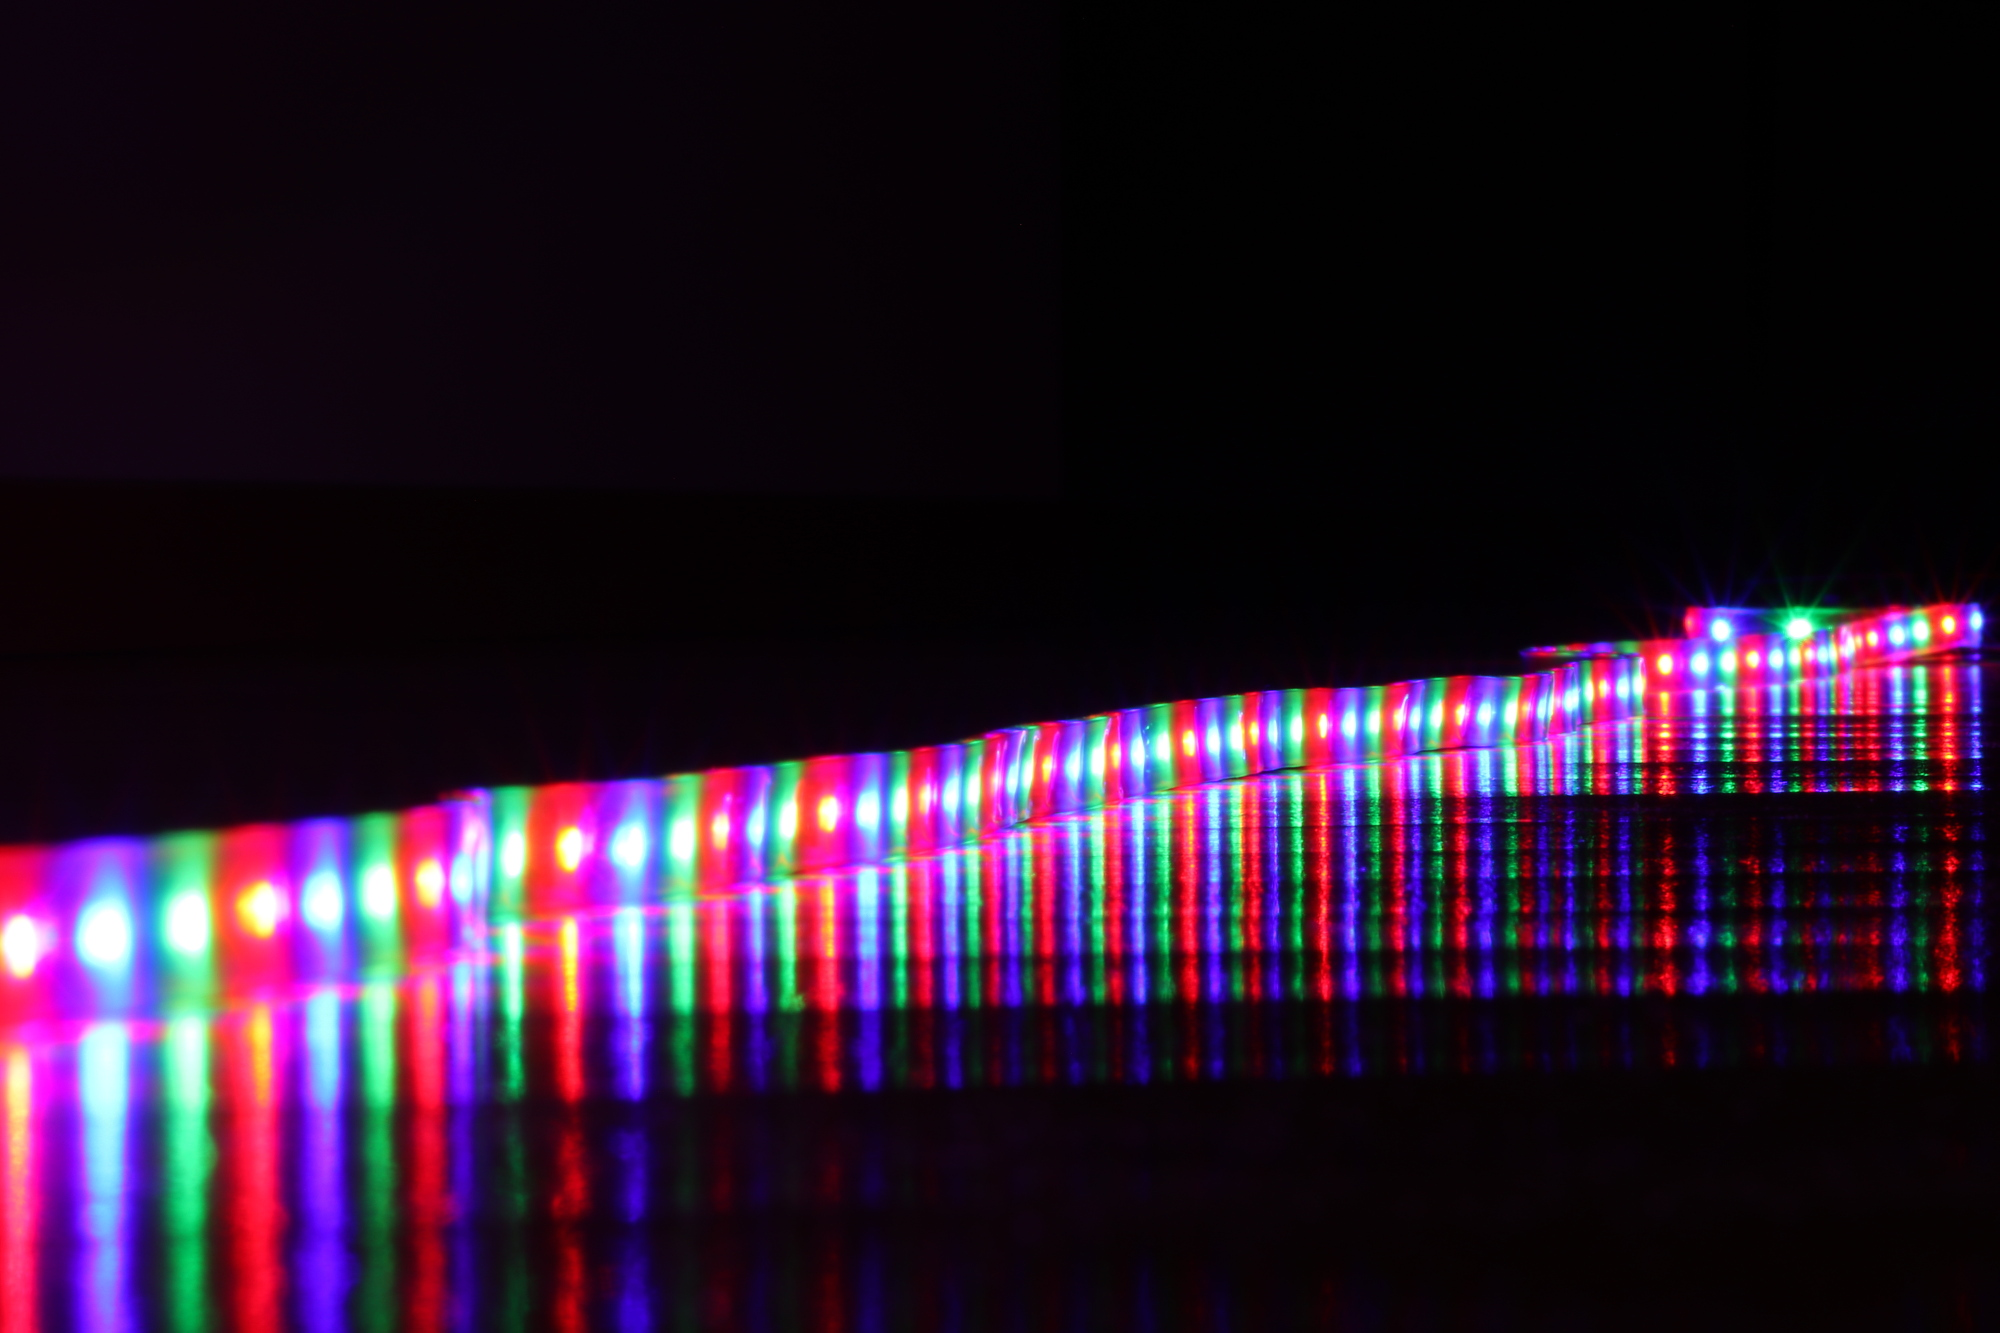
\includegraphics{../pictures/title_klein.JPG}
\caption{Titelbild}
\end{figure}

\subsection{Gruppe}\label{gruppe}

\begin{itemize}
\item
  Andreas Züger
\item
  Markus Schenk
\item
  \sout{Endre Marczi}
\end{itemize}

\subsection{Abstract}\label{abstract}

Das Projekt WakeUp-Light erstellt ein Wecksystem dass mittels einem
zentralen Server und einem REST-WebService gesteuert werden kann. Der
Benutzer des Systems kann Wecker konfigurieren, mit denen er über eine
angegebene Weckzeit mit den konfigurierten Weckgeräten geweckt wird. Der
zentrale Server stellt die Weckinformationen mittels einem
REST-WebService seinen Clients zur Verfügung. Die Clients übernehmen die
Ansteuerung der angeschlossenen, externen (Weck-)Geräte und nehmen Input
von Sensoren entgegen. Beide Komponenten - der Server und die Clients -
sind auf einem oder mehreren Raspberry PI lauffähig.

\subsection{Analyse}\label{analyse}

\subsubsection{Problembeschreibung}\label{problembeschreibung}

Viele Menschen starten - gerade in den dunklen Wintermonaten - sehr
schlecht in den Tag, weil sie durch einen schrillen Weckton vor
Sonnenaufgang geweckt werden oder in einem ungünstigen Schlafrythmus
sind. Gerade Menschen mit einem späten Chronotypen fühlen sich dadurch
den ganzen Tag schläfrig und können oftmals weniger Leistung bringen.
Auch führt dies zu einer ungesunden Überzufuhr vom Wirkstoff Thein.

Der Markt hat auf diese Problematik mit sogenannten Wake-Up Lights
reagiert. Ein Wake-Up Light simuliert einen künstlichen Sonnenaufgang
auf die gewünschte Weckzeit hin und verspricht so einen natürlicheren
Aufwachvorgang. Die positive Wirksamkeit von Wake-Up Lights wurde auch
schon in einer Studie von Giménez {[}Gim{]} untersucht und aufgezeigt.

Die existierenden Produkte auf dem Markt sind meist stark eingebunden in
ein bestehendes Produktökosystem, was ihre Bedienung vereinfacht, aber
meist wenig Erweiterungs- und Anbindungsmöglichkeiten bietet.
Beispielsweise erlauben heutige Wake-Up Lights Weckmusik nur in
Kombination mit lokalen Musikdateien auf dem Smartphone oder mit
Musikdiensten.

\subsubsection{Vision}\label{vision}

Mit einem Raspberry Pi als Controller und einem LED-Strip wird ein
Wake-Up Light konzipiert und gebaut, das über ein GUI konfiguriert
werden kann. Der Benutzer kann das Wake-Up Light so einstellen, dass er
auf eine bestimmten Zeit hin geweckt wird. Zusätzlich soll das Wake-Up
Light mit schwachem Licht einschalten, wenn der Benutzer in der Nacht
aufsteht und das Zimmer verlässt. Die Software auf dem Raspberry Pi soll
ausserdem in Zukunft noch weitere - allenfalls bereits bestehende -
Geräte wie einen Receiver, oder Smart Lights ansprechen, um den
Weckvorgang noch weiter auf den Benutzer zuzuschneidern.

\subsubsection{Anforderungen}\label{anforderungen}

\begin{enumerate}
\def\labelenumi{\arabic{enumi}.}
\tightlist
\item
  Das Wake-Up Light dimmt ein Leuchtmittel über eine vorgegebene
  Zeitperiode.
\item
  Das Wake-Up Light reagiert bei Dunkelheit auf Bewegungen, und schaltet
  das Leuchtmittel im Nachtlichtmodus ein.
\end{enumerate}

\paragraph{Optional mit
Helligkeitssensor}\label{optional-mit-helligkeitssensor}

\begin{enumerate}
\def\labelenumi{\arabic{enumi}.}
\setcounter{enumi}{2}
\tightlist
\item
  Das Wake-Up Light schaltet das Leuchtmittel nur ein, wenn es nicht
  bereits hell in der Umgebung ist.
\end{enumerate}

\paragraph{Optional mit Taster}\label{optional-mit-taster}

\begin{enumerate}
\def\labelenumi{\arabic{enumi}.}
\setcounter{enumi}{3}
\tightlist
\item
  Das Wake-Up Light ist durch Knopfdruck einschaltbar und dient so als
  eine normale Zimmerbeleuchtung.
\end{enumerate}

\subsubsection{Kontextdiagramm}\label{kontextdiagramm}

\begin{figure}[H]
\centering
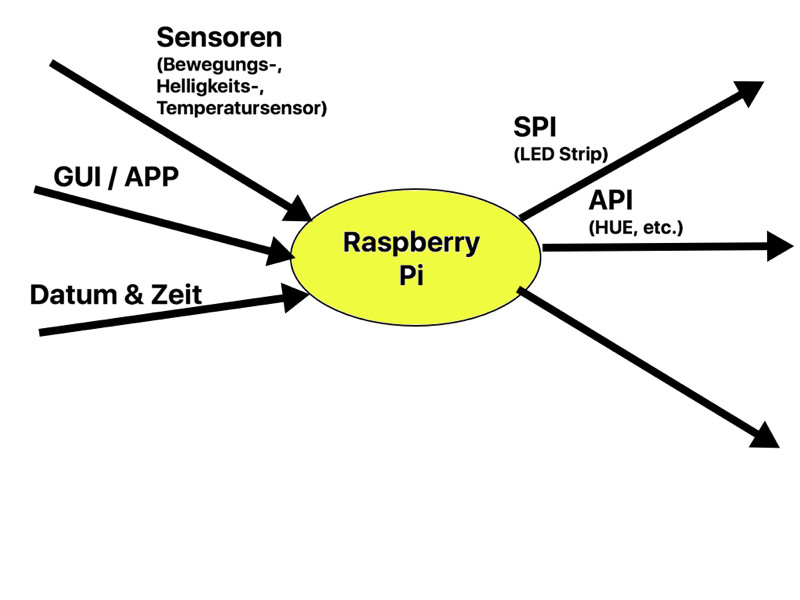
\includegraphics{./Kontextdiagramm.jpeg}
\caption{Kontextdiagramm Wake-Up Light}
\end{figure}

\subsubsection{Zeitplan}\label{zeitplan}

\paragraph{Rahmenbedingungen}\label{rahmenbedingungen}

\begin{itemize}
\tightlist
\item
  15.10.2016 : Abgabe Projektidee
\item
  05.11.2016 : Abgabe Kontextdiagramm, Anforderungsliste, Terminplan
\item
  19.11.2016 : Abgabe Schaltungsentwurf / Softwareentwurf / Testkonzept
\item
  03.12.2016 : Präsenz
\item
  03.01.2017 : Abgabe Dokumentation
\item
  14.01.2017 : Präsentation
\end{itemize}

\paragraph{Grobprojektplan}\label{grobprojektplan}

\begin{itemize}
\tightlist
\item
  15.10.2016 - 05.11.2016 : Analyse
\item
  06.11.2016 - 19.11.2016 : Design
\item
  20.11.2016 - 03.01.2017 : Implementation
\item
  04.01.2017 - 10.01.2017 : Testing
\item
  11.01.2017 - 13.01.2017 : Präsentation erstellen*
\end{itemize}

\subsection{Design}\label{design}

\subsubsection{Vorwort}\label{vorwort}

Das nachfolgende Designdokument soll die Anforderungen an das
WakeUp-Light, die in der Analyse definiert wurden, in umsetzbare
Spezifikationen manifestieren. Dazu werden die bereits gefundenen Use
Cases ausgebaut und mit Details angereichert, es werden erste
Klassendiagramme eingeführt, das Datenmodell und der WebService
spezifiziert und das Schaltbild wird zum ersten Mal präsentiert.

\subsubsection{Projektmanagement}\label{projektmanagement}

Um das Projekt WakeUp-Light besser zu koordinieren wurde das Vorhaben in
fünf Phasen gegliedert. 1. Analyse 2. Design 3. Implementierung 4. Test
5. Abgabe und Präsentation

Zu jeder Phase wurden terminierte und beschriebene Work Items erstellt.
Jedes Work Item stellt eine unabhängig, abschliessbare Arbeitseinheit
ein. Die Projektteilnehmer können sich für Work Items selbstständig
eintragen und sind dann dafür verantwortlich, sie bis zum Endtermin
abzuliefern. Zurzeit besteht das Projekt aus 49 Work Items die bis zum
Abschluss der Phase 3 reichen.

\begin{figure}[H]
\centering
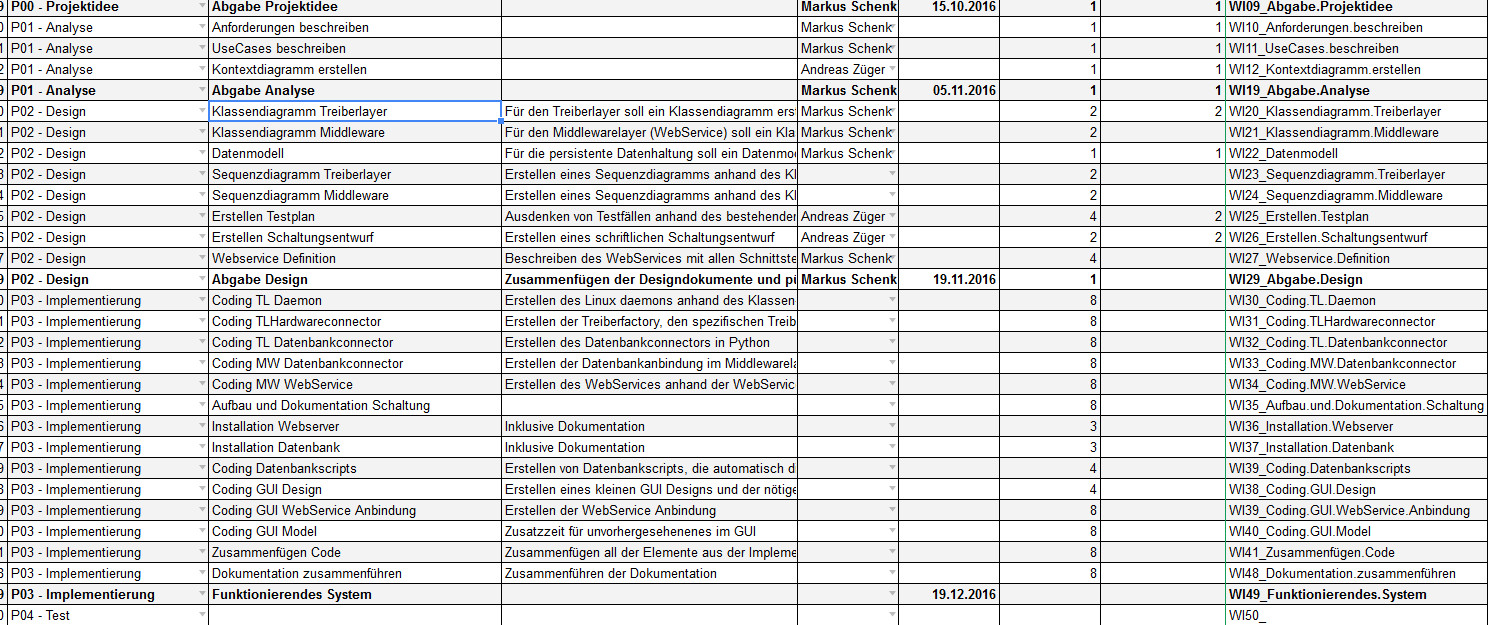
\includegraphics{./WI29_Abgabe_Design_Projektplan.jpeg}
\caption{Auszug Projektplan}
\end{figure}

\subsubsection{Use Case Diagramme}\label{use-case-diagramme}

Beim entwerfen der Klassendiagramme wurde auf den bestehenden Use Cases
aus der Analysephase aufgebaut. Die Use Cases wurden wo sinnvoll
erweitert, umbenannt oder ergänzt um möglichst stimmig für den
Endbenutzer und die Entwickler zu sein.

\begin{figure}[H]
\centering
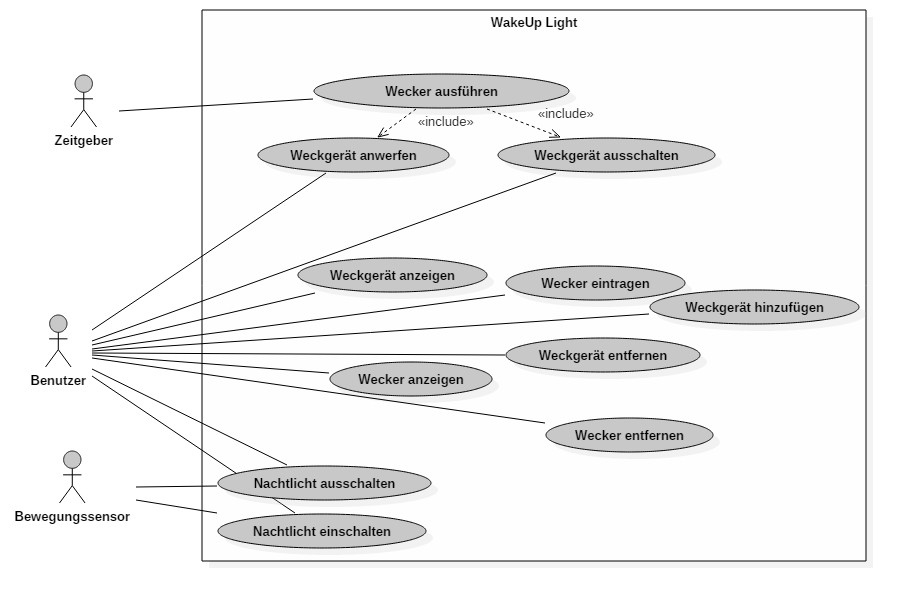
\includegraphics{./WI28_UseCase_Diagramm.jpeg}
\caption{WI28\_UseCase.Diagramm}
\end{figure}

\subsubsection{Datenmodell}\label{datenmodell}

Das Datenmodell stellt die persistente Datenhaltung in der Datenbank
dar. Der Treiberlayer zieht Aufträge aus der Datenbank und der
Middlewarelayer schreibt Aufträge in die Datenbank und liest
Informationen zur Anzeige aus der Datenbank.

\begin{figure}[H]
\centering
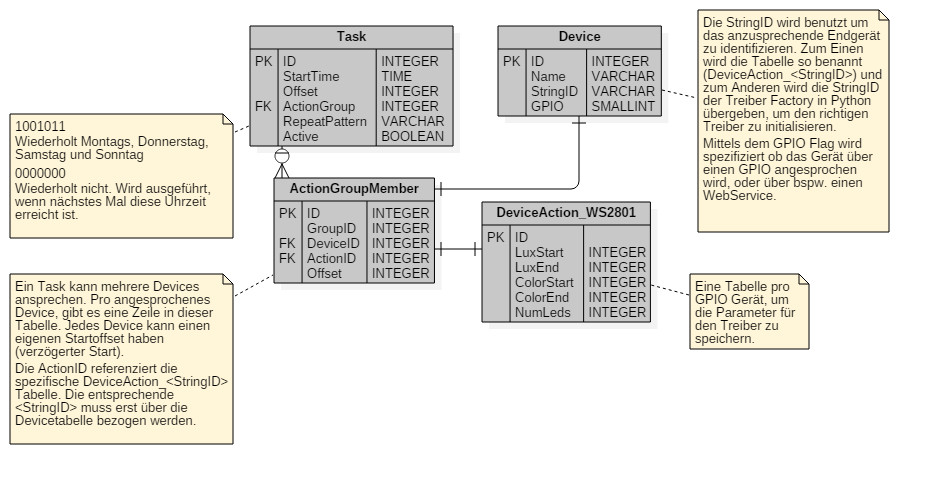
\includegraphics{./ERDDiagram.jpeg}
\caption{ERDDiagram}
\end{figure}

Für jedes anzusprechende Device gibt es einen Eintrag in der Tabelle
«Device». Dort wird ein ID-String abgelegt, über den man das Gerät auf
allen Schichten eindeutig identifizieren kann. Zu jeder Zeile in
«Device» gibt es eine eigene Tabelle «DeviceAction\_». Dort werden die
Parameter des Device abgelegt. Im Falle unseres LED-Strips sind das die
Start- und Endhelligkeit, die Start- und Endfarbe sowie die Anzahl der
LEDs (bzw. Pixel).

In der Tabelle «ActionGroupMember» werden die Geräte zu einer
ActionGroup zusammengefasst. Die Tabelle Task ruft also eine ActionGroup
auf und in der «ActionGroupMember» Tabelle gibt es für jedes Gerät, dass
zu diesem Task etwas ausführen soll, eine Zeile. In jeder Zeile kann ein
zusätzlicher Offset angegeben werden, wenn beispielsweise ein Gerät in
der ActionGroup erst später anlaufen soll.

\subsubsection{Definition Web Service}\label{definition-web-service}

Um zur Steuerung des WakeUp Lights nicht von einem spezifischen
Gerätetyp abhängig zu sein, werden die Steuerungsaufträge sowie die
Informationsabfragen über Web Service Abfragen getätigt. Dieser Web
Service wird hier zum ersten Mal spezifiziert. Die nachfolgenden
Klassendiagramme basieren auf dieser Spezifikation.

Die volle Spezifikation befindet sich in der Projektablage als
Excel-Datei.

\paragraph{Web Service Operations}\label{web-service-operations}

\begin{lstlisting}
GetDevice
AddDevice
RemoveDevice
GetAlarm
AddAlarm
RemoveAlarm
GetDeviceAction
AddDeviceAction
RemoveDeviceAction
GetActionGroupMember
AddActionGroupMember
RemoveActionGroupMember
ActivateActionGroup
DisableActionGroup
ActivateNightLight
DisableNightLight
\end{lstlisting}

\subparagraph{SOAP Requests}\label{soap-requests}

Nachfolgend ist eine Übersicht der zu den Operations gehörigen Requests
abgebildet. Das Bild ist ein statisches Beispiel. Die Dokumentation wird
in der Projektablage in der Excel-Datei nachgeführt.
\begin{figure}[H]
\centering
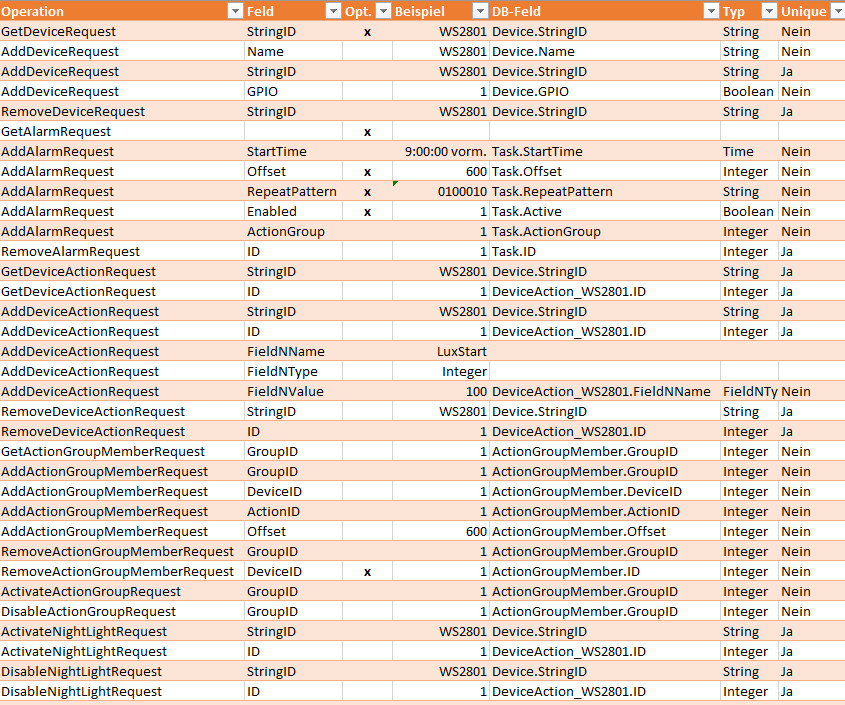
\includegraphics{./WI27_WebService_Definition_Requests.jpeg}
\caption{SOAP Requests}
\end{figure}

\subparagraph{SOAP Responses}\label{soap-responses}

Nachfolgend ist eine Übersicht der zu den Operations gehörigen Responses
abgebildet. Das Bild ist ein statisches Beispiel. Die Dokumentation wird
in der Projektablage in der Excel-Datei nachgeführt.
\begin{figure}[H]
\centering
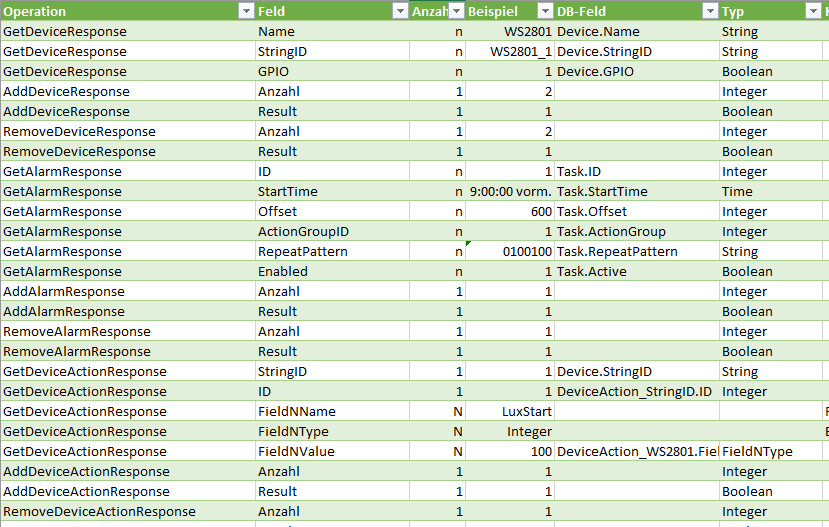
\includegraphics{./WI27_WebService_Definition_Responses.jpeg}
\caption{SOAP Responses}
\end{figure}

\newpage
\subsubsection{Klassendiagramme}\label{klassendiagramme}

Die nachfolgend gezeigten Klassendiagramme basieren auf dem oben
dargestellten Datenmodell sowie der Web Service Spezifikation.

\paragraph{Treiberlayer}\label{treiberlayer}

\begin{figure}[H]
\centering
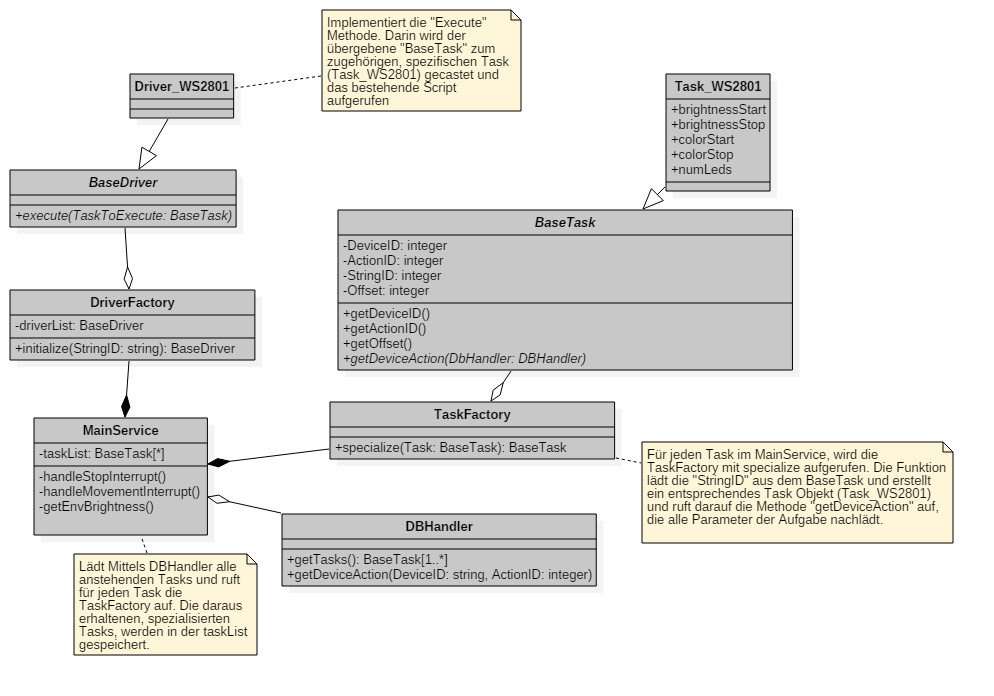
\includegraphics{./WI20_Klassendiagramm_Treiberlayer.jpeg}
\caption{Klassendiagramm Treiberlayer}
\end{figure}

Das Klassendiagramm sieht einen Linux-Daemon vor, der die Hauptlogik
enthält. Dieser erstellt einen DBHandler, der regelmässig alle Aufgaben
aus der Datenbank lädt. Der DBHandler selektiert alle Tasks die 1. Aktiv
sind, 2. Die Uhrzeit erreicht ist, 3. Das RepeatingPattern erfüllt ist
und 4. Deren Devices in der ActionGroup GPIO relevant sind

und schickt diese an den MainService als «BaseTask» zurück. Jetzt wird
ein Task für jedes anzusprechende Device erstellt. Der MainService ruft
für jeden so erstellten Task, die TaskFactory mit «specialize» auf.
«Specialize» versucht anhand der StringID, das richtige POCO-Objekt zu
erstellen (Task\_WS2801) und gibt dieses zurück. Dieses Objekt wird nun
im MainService in der «taskList» abgespeichert. Für jeden Task in der
taskList wird nun die DriverFactory mit der StringID des Tasks
aufgerufen. Die DriverFactory versucht das richtige Driver-Objekt zu
erstellen («Driver\_WS2801») und gibt dieses als BaseDriver Objekt
zurück. Der MainService ruft nun auf dem BaseDriver-Objekt mittels
Polymorphismus die «execute» Funktion auf. Die Execute-Funktion ist in
jedem expliziten Driver «Driver\_WS2801» implementiert und enthält den
Scriptaufruf mit den Angaben aus dem jeweiligen Task (Task\_WS2801)
Objekt.

\paragraph{Middlewarelayer}\label{middlewarelayer}

\begin{figure}[H]
\centering
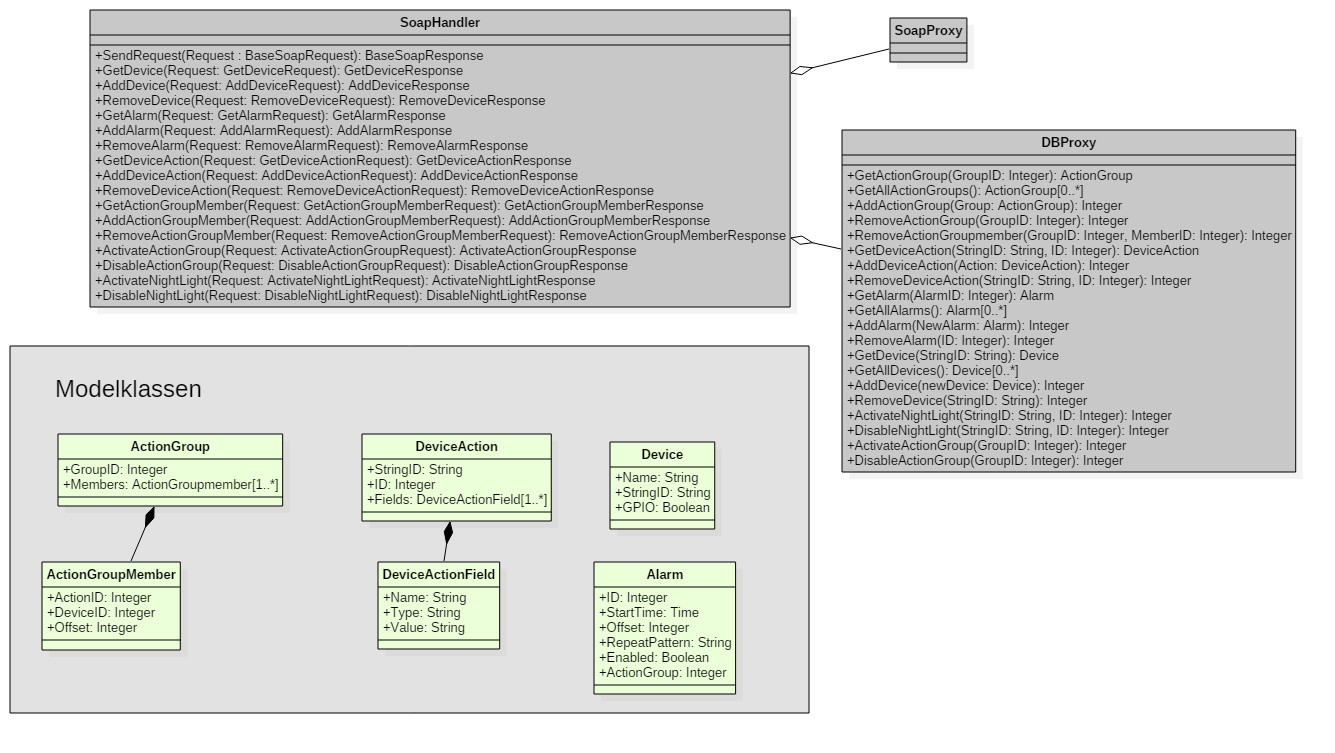
\includegraphics{./WI21_Klassendiagramm_Middleware.jpeg} 
\caption{Klassendiagramm Middleware}
\end{figure} 
Der SoapHandler schickt bei Bedarf WebService Requests an Komponenten die per Web
Service angebunden sind (LIFX) und empfängt WebService Requests, die für
das WakeUp-Light gedacht sind. Er implementiert die oben spezifizierten
WebService Operationen.

Der DBProxy übernimmt die Kommunikation zur Datenbank. Der SoapHandler
ist dafür zuständig, dass er seine Requests richtig interpretiert und
die richtige Funktion auf dem DBProxy aufruft.

Der SoapProxy übernimmt die tatsächlichen Verbindungsdetails und
Netzwerktechnischen Details. Dieser wird hier nicht weiter ausgeführt,
da er für die Funktionsweise der Endsoftware irrelevant ist.

\subsubsection{Testplan}\label{testplan}

Die im Design ausgearbeitete Spezifikation beinhaltet bereits einiges an
Funktionalität. Um diese Funktionalität testen zu können, wurde ein
spezifischer Testplan erstellt, der die in der Analyse und dem Design
ausgearbeiteten Features abdecken soll. Der Testplan wird im
Projektrepository als Excel-Datei geführt und ist hier nur auszugsweise
als Beispiel aufgeführt.

\begin{figure}[H]
\centering
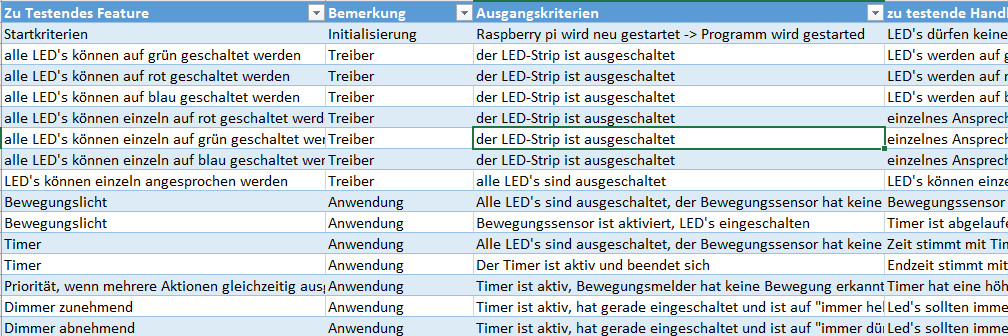
\includegraphics{./WI25_Erstellen_Testplan_Auszug.jpeg}
\caption{Auszug aus dem Testplan}
\end{figure}

\subsubsection{Schaltungsentwurf}\label{schaltungsentwurf}

Die Schaltung zeigt, wie das Hauptweckmedium (die LED-Pixelkette WS2801)
an den Raspberry PI angeschlossen wird. Die Applikation sieht vor, dass
auch andere Geräte angeschlossen und angesteuert werden können.

\begin{figure}[H]
\centering
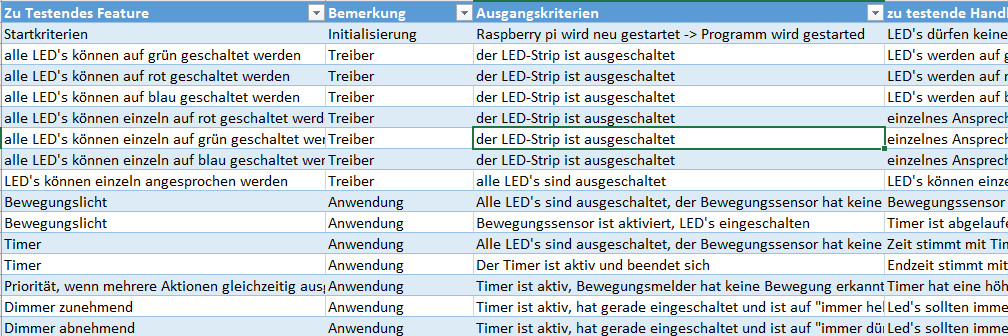
\includegraphics{./WI25_Erstellen_Testplan_Auszug.jpeg}
\caption{Schaltungsentwurf}
\end{figure}

\subsection{Implementation}\label{implementation}

\subsubsection{Umstellung von SOAP auf
REST}\label{umstellung-von-soap-auf-rest}

Nach dem Design im Team entschieden den WebService - anstatt wie in der
Analyse angedacht mit SOAP - in REST zu implementieren. Dies weil zu
diesem Zeitpunkt das Projekt noch ein Teammitglied hatte, das sich nur
mit REST WebServices auskannte. Daher wurde die WebService Spezifikation
ebenfalls von SOAP auf REST umgeschrieben.

\paragraph{Web Service Operations}\label{web-service-operations-1}

\begin{itemize}
\tightlist
\item
  /api/devices
\item
  /api/alarms
\item
  /api/deviceactions
\item
  /api/actiongroupmembers
\item
  /api/actiongroup/activate
\item
  /api/actiongroup/disable
\item
  /api/nightlight/activate
\item
  /api/nightlight/disable
\end{itemize}

\subparagraph{GET Operations}\label{get-operations}

Nachfolgend ist eine Übersicht der zu den Operations gehörigen
GET-Requests abgebildet. Das Bild ist ein statisches Beispiel. Die
Dokumentation wird in der Projektablage in der Excel-Datei nachgeführt.
\begin{figure}[H]
\centering
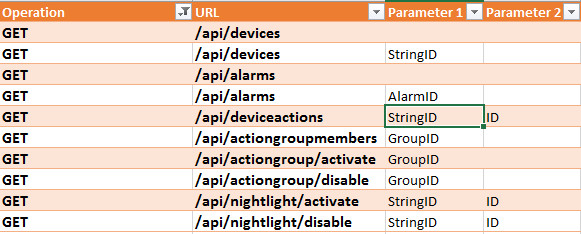
\includegraphics{./WI27_WebService_Definition_GET.jpeg}
\caption{REST GET Requests}
\end{figure}


\subparagraph{POST Operations}\label{post-operations}

Nachfolgend ist eine Übersicht der zu den Operations gehörigen
POST-Requests abgebildet. Das Bild ist ein statisches Beispiel. Die
Dokumentation wird in der Projektablage in der Excel-Datei nachgeführt.
\begin{figure}[H]
\centering
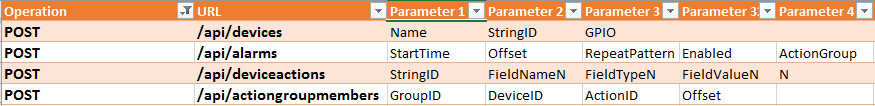
\includegraphics{./WI27_WebService_Definition_POST.jpeg}
\caption{REST POST Requests}
\end{figure}

\subparagraph{DELETE Operations}\label{delete-operations}

Nachfolgend ist eine Übersicht der zu den Operations gehörigen
DELETE-Requests abgebildet. Das Bild ist ein statisches Beispiel. Die
Dokumentation wird in der Projektablage in der Excel-Datei nachgeführt.
\begin{figure}[H]
\centering
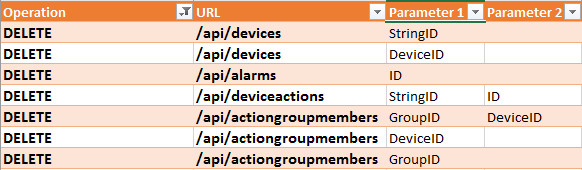
\includegraphics{./WI27_WebService_Definition_DELETE.jpeg}
\caption{REST DELETE Requests}
\end{figure}


\subsubsection{Aktualisierte
Klassendiagramme}\label{aktualisierte-klassendiagramme}

\paragraph{Middlewarelayer}\label{middlewarelayer-1}

\begin{figure}[H]
\centering
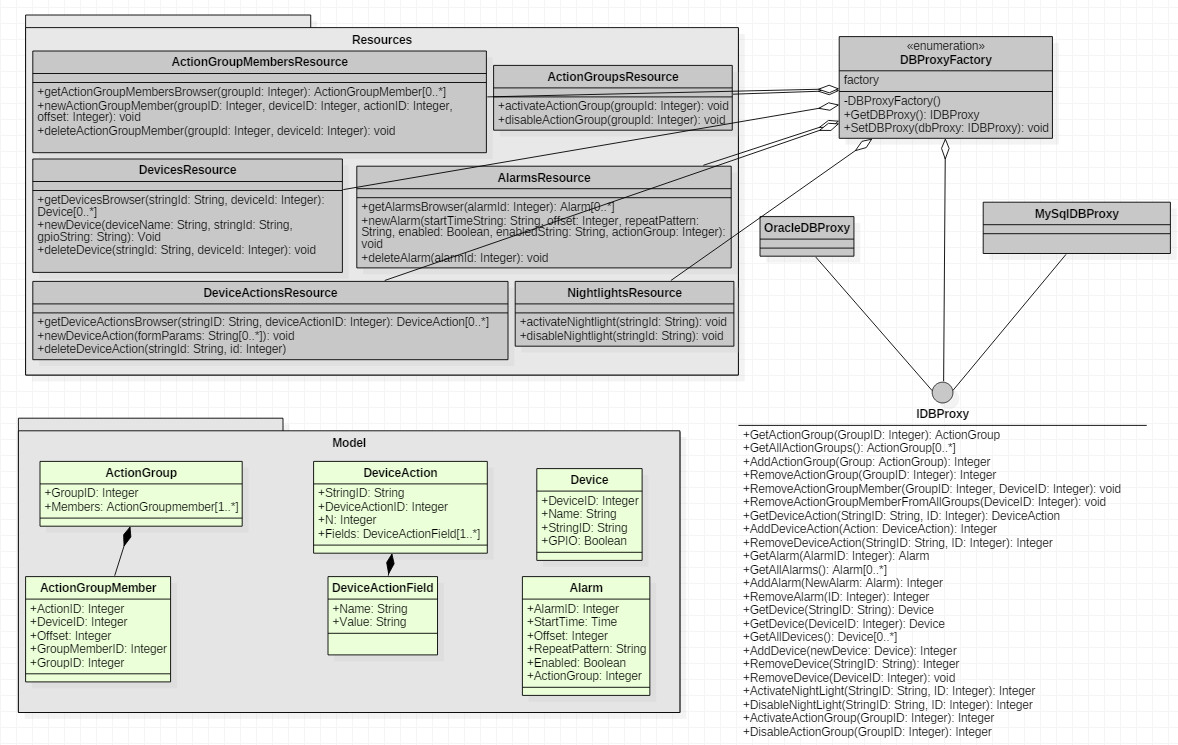
\includegraphics{./WI60_Nachfuehren_Design_Middleware.jpeg}
\caption{Aktualisiertes Middleware Design}
\end{figure}

\textbf{Resources}\\
Die Ressourcen sind die Endpunkte des REST Web Service. Für jede
ansprechbare Seite, existiert ein Endpunkt. Anfragen an diese Endpunkte
verarbeitet die JAX-RS Referenzimplementation Jersey und stellt die
jeweiligen Requestparameter mittels Autoboxing den Resource-Klassen zur
Verfügung. In diesen Resource-Klassen, sind dann die Java-Methoden
implementiert, die das tatsächliche ``doing'' auf Serverebene ausführen.

\textbf{DBProxyFactory}\\
Die DBProxyFactory hat die Aufgabe mittels Dependency Injection eine
Referenz auf einen gültigen \textbf{IDBProxy} zu produzieren. Die
Resource-Klassen greifen über die DBProxyFactory auf die
\textbf{IDBProxy} Instanz zu und kommunizieren so mit der Datenbank.
Dank dieser Indirektion erfüllt die Middleware das Dependency Inversion
Principle. Die DBProxyFactory ist ein Singleton als Enumeration
implementiert. Das hat den Vorteil, dass der Singleton auch nicht
mittels Reflection umgangen werden kann, sonst aber gleichwertig zum
klassischen Singleton ist.

\textbf{IDBProxy}\\
Das IDBProxy Interface implementiert die notwendigen Methoden um mit der
Datenbank zu kommunizieren. Eine Klasse, die das Interface
implementiert, muss nur noch Datenbankspezifisch die Methoden
implementieren.

\textbf{MySqlDBProxy}\\
In der tatsächlichen Implementation wird der SQL-Code umgesetzt, um die
im Interface spezifizierten Methoden auszühren. Im Wakeup-Light Projekt,
nutzt der finite DBProxy die Apache DbUtils für eine möglichst abstrakte
Datenbankkommunikation.

\textbf{Model}\\
Die Modelklassen sind die Mappingcontainer für die Verwendung der
relationalen Daten aus der Datenbank in der objekt-orientierten Welt.

\paragraph{Treiberlayer Model}\label{treiberlayer-model}

\begin{figure}[H]
\centering
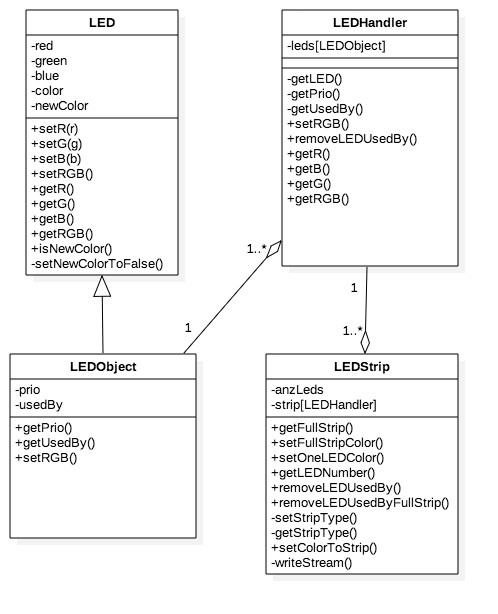
\includegraphics{./WI61_Treiber_Diagramm.jpeg}\\
\caption{Aktualisiertes Treiber Diagramm}
\end{figure}

\textbf{Klasse LED}\\
Beinhaltet die Grundlogik und Funktionen für jedes LED. Die Werte für
Rot, Grün, Blau können einzeln oder zusammen gesetzt werden. Zusätzlich
wird als Boolean abgespeichert ob eine neue Farbe gesetzt wurde. Nach
jedem abfragen der aktuellen Farbe wird der Boolean wieder auf False
gesetzt. So könnten theoretisch nur die LED's mit neuer Farbe
aktualisiert werden.

\textbf{Klasse LEDObject}\\
Diese Klasse erbt von die Grundfunktionen von der Klasse LED und
erweitert diese um die zwei Variablen „Priorität`` und „benutzt von``.
Idee dahinter ist, dass die Timer unterschiedliche Prioriät haben. So
ist bspw. das Nachtlicht sekundär und hat darum eine niedriegere Prio.
Ist nun ein Timer aktiv, kann das Nachtlicht ebenfalls reagieren, es
ändert aber nichts an der Farben des Strips, da der Timer höherrangig
ist.

\textbf{Klasse LEDHandler}\\
Die Klasse enhält ein Array von LEDObject's. Somit kann für jeden Aufruf
für verschiedene Timer oder andere aktivitäten ein LED mit Farbe,
Priorität und ID des Aufrufers abgespeichert werden. Wird nun der Strip
„geschrieben`` also physisch angezeigt, wird für jedes einzelne LED die
Farbe Aufrufs mit der höchsten Prio angezeigt. Ist z.B. ein Timer
beendet, kann mittels der Funktion removeLEDUsedBy() das LED gelöscht
werden und das LED mit der nächst tieferen Prio wird angezeigt.

\textbf{Klasse LEDStrip}\\
LEDStrip bildet den pyhsischen Strip ab. Die Klasse besitzt ein Array
mit der Anzahl LEDHandler wie LED's am Strip sind. Es ist möglich dem
ganzen Strip die gleiche Farbe zu geben, sowie auch nur einzelne LED's
zu beeinflussen. Mittels der Funktion setColorToStrip() wird der Strip
aktualisiert.

\paragraph{Treiberlayer Middlelayer}\label{treiberlayer-middlelayer}

\begin{figure}[H]
\centering
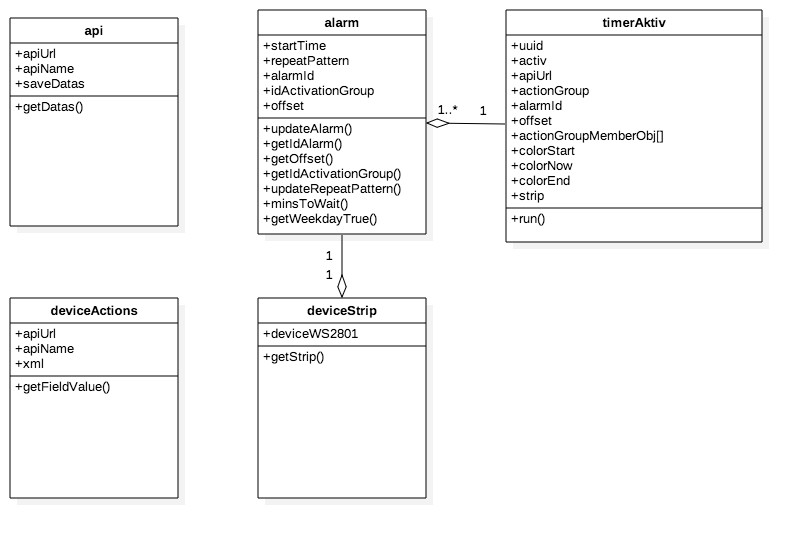
\includegraphics{./WI61DriverMiddlelayer.jpeg}
\caption{Aktualisiertes Diagramm Treiberwrapper}
\end{figure}

 \textbf{Treiberwrapper}\\
Über die API-Klasse werden die Daten der DB Abgefragt. Alle Requests
greifen auf die API's zu. Ursprünglich war vorgesehen, die Daten direkt
aus der Datenbank zu beziehen. Dies hätte aber dazu geführt, dass die
Weckgeräte stark an die Datenbank gekoppelt gewesen wären - und ein
Architekturwechsel in der Datenbank immer Folgen für jedes Weckgerät
gehabt hätte. Tests mit dem Web Service haben gezeigt, dass dieser
schnell und zuverlässig genug reagiert, dass die Weckgeräte ihre Daten
ebenfalls darüber beziehen können. Für jede der einzelnen API's wurde
eine Hilfsklasse erstellt, damit die Daten einfach gespeichert und
abgefragt werden können. Zusätzlich existiert eine Klasse Alarm. In
dieser wird der Alarm abgebildet.

Das folgende Ablaufdiagramm zeigt, wie der Treiberlayer entscheidet, ob
eines seiner angeschlossenen Geräte jetzt aktiviert werden soll.

\begin{figure}[H]
\centering
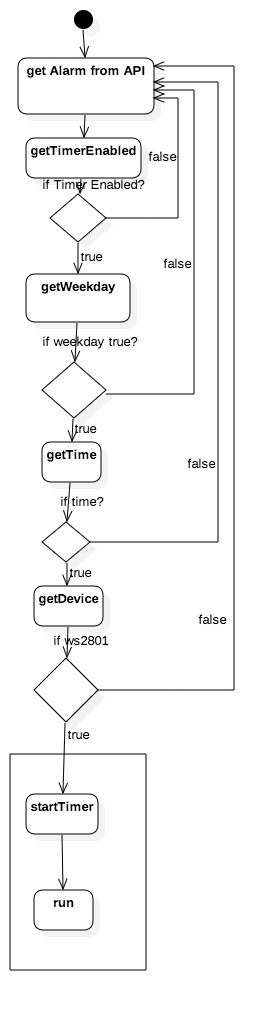
\includegraphics[width=6in,height=6in]{./WI61ActivityDiagramm.jpeg}
\caption{Beispiel Activity Diagram}
\end{figure}

\subsubsection{Verwendete Frameworks, Abhängigkeiten und
Libraries}\label{verwendete-frameworks-abhuxe4ngigkeiten-und-libraries}

Zur Effizienten Umsetzung wurden Libraries und Frameworks eingesetzt.
Nachfolgend sind diese externen Abhängigkeiten nach Layer aufgeteilt
aufgelistet.

\paragraph{Middleware}\label{middleware}

\begin{itemize}
\tightlist
\item
  Jersey (JAX-RS Reference Implementation)
\item
  DbUtils (Apache Commons, JDBC Utility Component)
\item
  Tomcat 8 (Applicationserver)
\item
  Java Runtime Environment
\end{itemize}

\paragraph{Treiberlayer}\label{treiberlayer-1}

\begin{itemize}
\tightlist
\item
  Python2.7 (mit den Zusatzmodulen requests, xml.dom.minidom, xmltodict
  um die Api ansprechen zu können)
\end{itemize}

\subsubsection{Automatisierte
Installation}\label{automatisierte-installation}

Um die Serverinstallation zu vereinfachen, wurde ein Installationsscript
in Shell-Script erstellt, dass die Serverinstallation und das Deployment
auf dem Raspberry-PI komplett automatisiert durchführt.

Das Script initialisiert erst einige Variablen, damit bei Änderungen
nicht das ganze Script nicht durchsucht werden muss.

\begin{minted}{bash}
#!/bin/bash

mysql_version="mysql-server"
tomcat_version="tomcat8"
java_version="oracle-java8-installer"

context="ROOT"
sqlFile="02_SQL/WI39_Coding.Datenbankscripts.sql"
warFile="03_Middleware/ROOT.war"

JAVA_HOME="/usr/lib/jvm/java-8-oracle"
CATALINA_HOME="/usr/share/$tomcat_version"
CATALINA_BASE="/var/lib/$tomcat_version"
\end{minted}

Die Funktion canDownload überprüft, ob ein zu installierendes Paket
überhaupt verfügbar ist. Die Funktion isInstalled prüft, ob ein
entsprechendes Paket nicht bereits installiert ist.

Damit Software installiert werden kann, muss das Script mit ROOT-Rechten
aufgerufen werden. Das Script überprüft, ob der aufrufende User
ROOT-Rechte hat, bevor es weitermacht.

Als ersten Parameter erwartet das Script den Pfad zum Server-WAR-File
das deployed werden soll.

\begin{minted}{bash}
canDownload()
{
  if [[ $(apt-cache search $1 | wc -l) -gt 0 ]] ; then { return 0; } fi
  return 1
}

isInstalled()
{
  if [[ $(dpkg -l | grep $1 | wc -l) -gt 0 ]] ; then { return 0; } fi
  return 1
}

if [[ "$EUID" -ne 0 ]] ; then
  echo "Please run as root"
  exit
fi

if [ ! -f $1 ] || [ -z ${1+x} ] ; then
  echo "Pass WAR-File as first parameter"; 
  exit 1
fi

warFile=$1
\end{minted}

Damit die offizielle Oracle JVM installiert werden kann, muss eine
zusätzliche Quelle hinzugefügt werden und der entsprechende public key
installiert werden.

\begin{minted}{bash}
echo "deb http://ppa.launchpad.net/webupd8team/java/ubuntu trusty main" > /etc/apt/sources.list.d/webupd8team-java.list
echo "deb-src http://ppa.launchpad.net/webupd8team/java/ubuntu trusty main" >> /etc/apt/sources.list.d/webupd8team-java.list
apt-key adv --keyserver keyserver.ubuntu.com --recv-keys EEA14886
\end{minted}

Das Script führt nun einen Quellen Update durch und installiert die
debconf-utils damit nachfolgende Konfigurationen der Installationen
einfacher durchgeführt werden können.

\begin{minted}{bash}
apt-get -y -qq  update
apt-get -y -qq  install debconf-utils
\end{minted}

Nun werden nacheinander die benötigten Tools installiert. Das Script
prüft jeweils erst ob es heruntergeladen werden kann, bevor es
tatsächlich etwas versucht zu installieren. Nach der Installation prüft
das Script, ob die Installation geklappt hat. Wenn nicht, bricht es ab.

\begin{minted}{bash}
if ! canDownload $java_version || ! canDownload $mysql_version || ! canDownload $tomcat_version ; then
  echo "Could not download necessary software. Aborting."
  exit 1
fi

if ! isInstalled $java_version ; then
  echo "installing $java_version..."
  debconf-set-selections <<< "debconf shared/accepted-oracle-license-v1-1 select true"
  debconf-set-selections <<< "debconf shared/accepted-oracle-license-v1-1 seen true"
  apt-get -y -qqq install $java_version > /dev/null

  export JAVA_HOME

  if ! isInstalled $java_version ; then
    echo "Could not install $java_version. Aborting."
    exit 1; 
  fi
fi
\end{minted}

Tomcat wird als Application Server benutzt, der den REST-WebService
hosted. Das Script versucht hier diesen zu installieren und führt einige
Basiskonfigurationen durch.

\begin{minted}{bash}
if ! isInstalled $tomcat_version ; then
  echo "adding tomcat user..."
  adduser --quiet --system --shell /bin/bash --gecos 'Tomcat Java Servlet and JSP engine' --group --disabled-password --home /home/tomcat $tomcat_version

  echo "installing $tomcat_version..."
  apt-get -y -qq install $tomcat_version > /dev/null

  export CATALINA_HOME
  echo "export CATALINA_BASE=$CATALINA_BASE" >> $CATALINA_HOME/bin/setenv.sh
  chown $tomcat_version:$tomcat_version $CATALINA_HOME/bin/setenv.sh
  chmod a+x $CATALINA_HOME/bin/setenv.sh
  mkdir $CATALINA_BASE/temp
  chown $tomcat_version:$tomcat_version $CATALINA_BASE/temp

  sed -i "s:#JAVA_HOME=.*:JAVA_HOME=$JAVA_HOME:" /etc/default/$tomcat_version

  if ! isInstalled $tomcat_version  ; then
  echo "Could not install $tomcat_version. Aborting."
  exit 1; 
  fi
fi
\end{minted}

In dieser Präsentationskonfiguration wird MySQL als DBMS eingesetzt.
Dieser wird hier installiert.

\begin{minted}{bash}
if ! isInstalled $mysql_version ; then
  echo "installing $mysql_version..."
  debconf-set-selections <<< "$mysql_version mysql-server/root_password password eshh"
  debconf-set-selections <<< "$mysql_version mysql-server/root_password_again password eshh"
  apt-get -y -qq install $mysql_version > /dev/null

  if ! isInstalled $mysql_version ; then
  echo "Could not install $mysql_version. Aborting."
  exit 1; 
  fi
fi
\end{minted}

Nun führt das Script eine rudimentäre Konfiguration des MySQL-Server
durch und importiert die Testdaten in die Datenbank. Ausserdem wird das
mitgegebene WAR-File deployed.

\begin{minted}{bash}
ip=$(hostname -I)
echo "[mysqld]"  > /etc/mysql/conf.d/wakeuplight.cnf
echo "bind-address   = $ip" >> /etc/mysql/conf.d/wakeuplight.cnf

echo "adding test data to database mydb..."
mysql --user=root --password=eshh < $sqlFile

rm -rf $CATALINA_BASE/webapps/$context
rm -rf $CATALINA_BASE/webapps/$context.war
cp $warFile $CATALINA_BASE/webapps/$context.war
chown -R $tomcat_version:$tomcat_version $CATALINA_BASE/webapps

systemctl restart $tomcat_version

### Installing Python Tools
echo "install python pip, xmltodict"
sudo apt-get -y -qq install python-pip
sudo pip -q install xmltodict

### summary
echo "All finished!"
echo "MySQL ist available at $ip on port 3306, use the wakeuplight user!"
echo "REST API is available at $ip:8080/rest/"
\end{minted}

\subsection{Tests}\label{tests}

Alle Testszenarios wurden durchgespielt. Für die Treibertests wurde ein
Skript (testplan.py) angelegt welches die Tests nacheinander durchläuft.
Jedes LED lässt sich einzeln steuern. Zusätzlich wurde mit weiteren
Tests die Prioritätsfunktion überprüft (wenn mehrere Programme
gleichzeitig aktiv sind). Werden für die LED's verschiedene Prio's mit
verschiedenen Farben festgelegt, erscheinen auch die geforderten Farben.
Sobald eine Farbe gelöscht wird, erscheint die Farbe mit der nächst
tieferen Prio. Da der Strip als Singleton implementiert wurde, kann man
auch sicher sein, dass immer der gleiche Strip angesprochen wird.

\begin{longtable}[]{@{}lc@{}}
\toprule
\begin{minipage}[b]{0.25\columnwidth}\raggedright\strut
Testnummer\strut
\end{minipage} & \begin{minipage}[b]{0.55\columnwidth}\centering\strut
1\strut
\end{minipage}\tabularnewline
\midrule
\endhead
\begin{minipage}[t]{0.25\columnwidth}\raggedright\strut
zu testendes Feature\strut
\end{minipage} & \begin{minipage}[t]{0.55\columnwidth}\centering\strut
Startkriterien\strut
\end{minipage}\tabularnewline
\begin{minipage}[t]{0.25\columnwidth}\raggedright\strut
Bemerkung\strut
\end{minipage} & \begin{minipage}[t]{0.55\columnwidth}\centering\strut
Initialisierung\strut
\end{minipage}\tabularnewline
\begin{minipage}[t]{0.25\columnwidth}\raggedright\strut
Ausgangskriterien\strut
\end{minipage} & \begin{minipage}[t]{0.55\columnwidth}\centering\strut
Raspberry pi wird neu gestartet -\textgreater{} Programm wird
gestarted\strut
\end{minipage}\tabularnewline
\begin{minipage}[t]{0.25\columnwidth}\raggedright\strut
zu testende Handlung\strut
\end{minipage} & \begin{minipage}[t]{0.55\columnwidth}\centering\strut
LED's dürfen keine undefinierten Werte / Farben haben\strut
\end{minipage}\tabularnewline
\begin{minipage}[t]{0.25\columnwidth}\raggedright\strut
erwartete Reaktion\strut
\end{minipage} & \begin{minipage}[t]{0.55\columnwidth}\centering\strut
LED's werden korrekt initialisiert und ausgeschaltet\strut
\end{minipage}\tabularnewline
\begin{minipage}[t]{0.25\columnwidth}\raggedright\strut
tatsächliche Reaktion\strut
\end{minipage} & \begin{minipage}[t]{0.55\columnwidth}\centering\strut
wie erwartet\strut
\end{minipage}\tabularnewline
\begin{minipage}[t]{0.25\columnwidth}\raggedright\strut
Fazit\strut
\end{minipage} & \begin{minipage}[t]{0.55\columnwidth}\centering\strut
Led's werden zur Sicherheit bei jedem Start der Software neu
initalisiert und ausgeschaltet. Funktioniert\strut
\end{minipage}\tabularnewline
\bottomrule
\end{longtable}

\begin{longtable}[]{@{}lc@{}}
\toprule
\begin{minipage}[b]{0.25\columnwidth}\raggedright\strut
Testnummer\strut
\end{minipage} & \begin{minipage}[b]{0.55\columnwidth}\centering\strut
2\strut
\end{minipage}\tabularnewline
\midrule
\endhead
\begin{minipage}[t]{0.25\columnwidth}\raggedright\strut
zu testendes Feature\strut
\end{minipage} & \begin{minipage}[t]{0.55\columnwidth}\centering\strut
alle LED's können auf grün geschaltet werden\strut
\end{minipage}\tabularnewline
\begin{minipage}[t]{0.25\columnwidth}\raggedright\strut
Bemerkung\strut
\end{minipage} & \begin{minipage}[t]{0.55\columnwidth}\centering\strut
Treiber\strut
\end{minipage}\tabularnewline
\begin{minipage}[t]{0.25\columnwidth}\raggedright\strut
Ausgangskriterien\strut
\end{minipage} & \begin{minipage}[t]{0.55\columnwidth}\centering\strut
der LED-Strip ist ausgeschaltet\strut
\end{minipage}\tabularnewline
\begin{minipage}[t]{0.25\columnwidth}\raggedright\strut
zu testende Handlung\strut
\end{minipage} & \begin{minipage}[t]{0.55\columnwidth}\centering\strut
Alle LED's werden auf grün geschaltet ( über Konsole )\strut
\end{minipage}\tabularnewline
\begin{minipage}[t]{0.25\columnwidth}\raggedright\strut
erwartete Reaktion\strut
\end{minipage} & \begin{minipage}[t]{0.55\columnwidth}\centering\strut
alle LED's leuchten grün\strut
\end{minipage}\tabularnewline
\begin{minipage}[t]{0.25\columnwidth}\raggedright\strut
tatsächliche Reaktion\strut
\end{minipage} & \begin{minipage}[t]{0.55\columnwidth}\centering\strut
wie erwartet\strut
\end{minipage}\tabularnewline
\begin{minipage}[t]{0.25\columnwidth}\raggedright\strut
Fazit\strut
\end{minipage} & \begin{minipage}[t]{0.55\columnwidth}\centering\strut
Funktioniert\strut
\end{minipage}\tabularnewline
\bottomrule
\end{longtable}

\begin{longtable}[]{@{}lc@{}}
\toprule
\begin{minipage}[b]{0.25\columnwidth}\raggedright\strut
Testnummer\strut
\end{minipage} & \begin{minipage}[b]{0.55\columnwidth}\centering\strut
3\strut
\end{minipage}\tabularnewline
\midrule
\endhead
\begin{minipage}[t]{0.25\columnwidth}\raggedright\strut
zu testendes Feature\strut
\end{minipage} & \begin{minipage}[t]{0.55\columnwidth}\centering\strut
alle LED's können auf rot geschaltet werden\strut
\end{minipage}\tabularnewline
\begin{minipage}[t]{0.25\columnwidth}\raggedright\strut
Bemerkung\strut
\end{minipage} & \begin{minipage}[t]{0.55\columnwidth}\centering\strut
Treiber\strut
\end{minipage}\tabularnewline
\begin{minipage}[t]{0.25\columnwidth}\raggedright\strut
Ausgangskriterien\strut
\end{minipage} & \begin{minipage}[t]{0.55\columnwidth}\centering\strut
der LED-Strip ist ausgeschaltet\strut
\end{minipage}\tabularnewline
\begin{minipage}[t]{0.25\columnwidth}\raggedright\strut
zu testende Handlung\strut
\end{minipage} & \begin{minipage}[t]{0.55\columnwidth}\centering\strut
Alle LED's werden auf rot geschaltet ( über Konsole )\strut
\end{minipage}\tabularnewline
\begin{minipage}[t]{0.25\columnwidth}\raggedright\strut
erwartete Reaktion\strut
\end{minipage} & \begin{minipage}[t]{0.55\columnwidth}\centering\strut
alle LED's leuchten rot\strut
\end{minipage}\tabularnewline
\begin{minipage}[t]{0.25\columnwidth}\raggedright\strut
tatsächliche Reaktion\strut
\end{minipage} & \begin{minipage}[t]{0.55\columnwidth}\centering\strut
wie erwartet\strut
\end{minipage}\tabularnewline
\begin{minipage}[t]{0.25\columnwidth}\raggedright\strut
Fazit\strut
\end{minipage} & \begin{minipage}[t]{0.55\columnwidth}\centering\strut
Funktioniert\strut
\end{minipage}\tabularnewline
\bottomrule
\end{longtable}

\begin{longtable}[]{@{}lc@{}}
\toprule
\begin{minipage}[b]{0.25\columnwidth}\raggedright\strut
Testnummer\strut
\end{minipage} & \begin{minipage}[b]{0.55\columnwidth}\centering\strut
4\strut
\end{minipage}\tabularnewline
\midrule
\endhead
\begin{minipage}[t]{0.25\columnwidth}\raggedright\strut
zu testendes Feature\strut
\end{minipage} & \begin{minipage}[t]{0.55\columnwidth}\centering\strut
alle LED's können auf blau geschaltet werden\strut
\end{minipage}\tabularnewline
\begin{minipage}[t]{0.25\columnwidth}\raggedright\strut
Bemerkung\strut
\end{minipage} & \begin{minipage}[t]{0.55\columnwidth}\centering\strut
Treiber\strut
\end{minipage}\tabularnewline
\begin{minipage}[t]{0.25\columnwidth}\raggedright\strut
Ausgangskriterien\strut
\end{minipage} & \begin{minipage}[t]{0.55\columnwidth}\centering\strut
der LED-Strip ist ausgeschaltet\strut
\end{minipage}\tabularnewline
\begin{minipage}[t]{0.25\columnwidth}\raggedright\strut
zu testende Handlung\strut
\end{minipage} & \begin{minipage}[t]{0.55\columnwidth}\centering\strut
Alle LED's werden auf blau geschaltet ( über Konsole )\strut
\end{minipage}\tabularnewline
\begin{minipage}[t]{0.25\columnwidth}\raggedright\strut
erwartete Reaktion\strut
\end{minipage} & \begin{minipage}[t]{0.55\columnwidth}\centering\strut
alle LED's leuchten blau\strut
\end{minipage}\tabularnewline
\begin{minipage}[t]{0.25\columnwidth}\raggedright\strut
tatsächliche Reaktion\strut
\end{minipage} & \begin{minipage}[t]{0.55\columnwidth}\centering\strut
wie erwartet\strut
\end{minipage}\tabularnewline
\begin{minipage}[t]{0.25\columnwidth}\raggedright\strut
Fazit\strut
\end{minipage} & \begin{minipage}[t]{0.55\columnwidth}\centering\strut
Funktioniert\strut
\end{minipage}\tabularnewline
\bottomrule
\end{longtable}

\begin{longtable}[]{@{}lc@{}}
\toprule
\begin{minipage}[b]{0.25\columnwidth}\raggedright\strut
Testnummer\strut
\end{minipage} & \begin{minipage}[b]{0.55\columnwidth}\centering\strut
5\strut
\end{minipage}\tabularnewline
\midrule
\endhead
\begin{minipage}[t]{0.25\columnwidth}\raggedright\strut
zu testendes Feature\strut
\end{minipage} & \begin{minipage}[t]{0.55\columnwidth}\centering\strut
alle LED's können einzeln auf rot geschaltet werden\strut
\end{minipage}\tabularnewline
\begin{minipage}[t]{0.25\columnwidth}\raggedright\strut
Bemerkung\strut
\end{minipage} & \begin{minipage}[t]{0.55\columnwidth}\centering\strut
Treiber\strut
\end{minipage}\tabularnewline
\begin{minipage}[t]{0.25\columnwidth}\raggedright\strut
Ausgangskriterien\strut
\end{minipage} & \begin{minipage}[t]{0.55\columnwidth}\centering\strut
der LED-Strip ist ausgeschaltet\strut
\end{minipage}\tabularnewline
\begin{minipage}[t]{0.25\columnwidth}\raggedright\strut
zu testende Handlung\strut
\end{minipage} & \begin{minipage}[t]{0.55\columnwidth}\centering\strut
einzelnes Ansprechen der LEDs mit rot ( über Konsole / Testscript
)\strut
\end{minipage}\tabularnewline
\begin{minipage}[t]{0.25\columnwidth}\raggedright\strut
erwartete Reaktion\strut
\end{minipage} & \begin{minipage}[t]{0.55\columnwidth}\centering\strut
jeweils ein nach dem anderen LED leuchtet rot\strut
\end{minipage}\tabularnewline
\begin{minipage}[t]{0.25\columnwidth}\raggedright\strut
tatsächliche Reaktion\strut
\end{minipage} & \begin{minipage}[t]{0.55\columnwidth}\centering\strut
wie erwartet\strut
\end{minipage}\tabularnewline
\begin{minipage}[t]{0.25\columnwidth}\raggedright\strut
Fazit\strut
\end{minipage} & \begin{minipage}[t]{0.55\columnwidth}\centering\strut
Das beschreiben des ganzen Strips dauert länger als erwartet, hier
sichtbar weil als Test ein ``lauflicht'' implementiert wurde\strut
\end{minipage}\tabularnewline
\bottomrule
\end{longtable}

\begin{longtable}[]{@{}lc@{}}
\toprule
\begin{minipage}[b]{0.25\columnwidth}\raggedright\strut
Testnummer\strut
\end{minipage} & \begin{minipage}[b]{0.55\columnwidth}\centering\strut
6\strut
\end{minipage}\tabularnewline
\midrule
\endhead
\begin{minipage}[t]{0.25\columnwidth}\raggedright\strut
zu testendes Feature\strut
\end{minipage} & \begin{minipage}[t]{0.55\columnwidth}\centering\strut
alle LED's können einzeln auf grün geschaltet werden\strut
\end{minipage}\tabularnewline
\begin{minipage}[t]{0.25\columnwidth}\raggedright\strut
Bemerkung\strut
\end{minipage} & \begin{minipage}[t]{0.55\columnwidth}\centering\strut
Treiber\strut
\end{minipage}\tabularnewline
\begin{minipage}[t]{0.25\columnwidth}\raggedright\strut
Ausgangskriterien\strut
\end{minipage} & \begin{minipage}[t]{0.55\columnwidth}\centering\strut
der LED-Strip ist ausgeschaltet\strut
\end{minipage}\tabularnewline
\begin{minipage}[t]{0.25\columnwidth}\raggedright\strut
zu testende Handlung\strut
\end{minipage} & \begin{minipage}[t]{0.55\columnwidth}\centering\strut
einzelnes Ansprechen der LEDs mit grün ( über Konsole / Testscript
)\strut
\end{minipage}\tabularnewline
\begin{minipage}[t]{0.25\columnwidth}\raggedright\strut
erwartete Reaktion\strut
\end{minipage} & \begin{minipage}[t]{0.55\columnwidth}\centering\strut
jeweils ein nach dem anderen LED leuchtet grün\strut
\end{minipage}\tabularnewline
\begin{minipage}[t]{0.25\columnwidth}\raggedright\strut
tatsächliche Reaktion\strut
\end{minipage} & \begin{minipage}[t]{0.55\columnwidth}\centering\strut
wie erwartet\strut
\end{minipage}\tabularnewline
\begin{minipage}[t]{0.25\columnwidth}\raggedright\strut
Fazit\strut
\end{minipage} & \begin{minipage}[t]{0.55\columnwidth}\centering\strut
Funktioniert\strut
\end{minipage}\tabularnewline
\bottomrule
\end{longtable}

\begin{longtable}[]{@{}lc@{}}
\toprule
\begin{minipage}[b]{0.25\columnwidth}\raggedright\strut
Testnummer\strut
\end{minipage} & \begin{minipage}[b]{0.55\columnwidth}\centering\strut
7\strut
\end{minipage}\tabularnewline
\midrule
\endhead
\begin{minipage}[t]{0.25\columnwidth}\raggedright\strut
zu testendes Feature\strut
\end{minipage} & \begin{minipage}[t]{0.55\columnwidth}\centering\strut
alle LED's können einzeln auf blau geschaltet werden\strut
\end{minipage}\tabularnewline
\begin{minipage}[t]{0.25\columnwidth}\raggedright\strut
Bemerkung\strut
\end{minipage} & \begin{minipage}[t]{0.55\columnwidth}\centering\strut
Treiber\strut
\end{minipage}\tabularnewline
\begin{minipage}[t]{0.25\columnwidth}\raggedright\strut
Ausgangskriterien\strut
\end{minipage} & \begin{minipage}[t]{0.55\columnwidth}\centering\strut
der LED-Strip ist ausgeschaltet\strut
\end{minipage}\tabularnewline
\begin{minipage}[t]{0.25\columnwidth}\raggedright\strut
zu testende Handlung\strut
\end{minipage} & \begin{minipage}[t]{0.55\columnwidth}\centering\strut
einzelnes Ansprechen der LEDs mit blau ( über Konsole / Testscript
)\strut
\end{minipage}\tabularnewline
\begin{minipage}[t]{0.25\columnwidth}\raggedright\strut
erwartete Reaktion\strut
\end{minipage} & \begin{minipage}[t]{0.55\columnwidth}\centering\strut
jeweils ein nach dem anderen LED leuchtet blau\strut
\end{minipage}\tabularnewline
\begin{minipage}[t]{0.25\columnwidth}\raggedright\strut
tatsächliche Reaktion\strut
\end{minipage} & \begin{minipage}[t]{0.55\columnwidth}\centering\strut
wie erwartet\strut
\end{minipage}\tabularnewline
\begin{minipage}[t]{0.25\columnwidth}\raggedright\strut
Fazit\strut
\end{minipage} & \begin{minipage}[t]{0.55\columnwidth}\centering\strut
Funktioniert\strut
\end{minipage}\tabularnewline
\bottomrule
\end{longtable}

\begin{longtable}[]{@{}lc@{}}
\toprule
\begin{minipage}[b]{0.25\columnwidth}\raggedright\strut
Testnummer\strut
\end{minipage} & \begin{minipage}[b]{0.55\columnwidth}\centering\strut
8\strut
\end{minipage}\tabularnewline
\midrule
\endhead
\begin{minipage}[t]{0.25\columnwidth}\raggedright\strut
zu testendes Feature\strut
\end{minipage} & \begin{minipage}[t]{0.55\columnwidth}\centering\strut
LED's können einzeln angesprochen werden\strut
\end{minipage}\tabularnewline
\begin{minipage}[t]{0.25\columnwidth}\raggedright\strut
Bemerkung\strut
\end{minipage} & \begin{minipage}[t]{0.55\columnwidth}\centering\strut
Treiber\strut
\end{minipage}\tabularnewline
\begin{minipage}[t]{0.25\columnwidth}\raggedright\strut
Ausgangskriterien\strut
\end{minipage} & \begin{minipage}[t]{0.55\columnwidth}\centering\strut
alle LED's sind ausgeschaltet\strut
\end{minipage}\tabularnewline
\begin{minipage}[t]{0.25\columnwidth}\raggedright\strut
zu testende Handlung\strut
\end{minipage} & \begin{minipage}[t]{0.55\columnwidth}\centering\strut
LED's können einzeln eingeschalten, gedimmt werden (über Konsole /
Testscript))\strut
\end{minipage}\tabularnewline
\begin{minipage}[t]{0.25\columnwidth}\raggedright\strut
erwartete Reaktion\strut
\end{minipage} & \begin{minipage}[t]{0.55\columnwidth}\centering\strut
Led's können einzeln gesteuert werden\strut
\end{minipage}\tabularnewline
\begin{minipage}[t]{0.25\columnwidth}\raggedright\strut
tatsächliche Reaktion\strut
\end{minipage} & \begin{minipage}[t]{0.55\columnwidth}\centering\strut
wie erwartet\strut
\end{minipage}\tabularnewline
\begin{minipage}[t]{0.25\columnwidth}\raggedright\strut
Fazit\strut
\end{minipage} & \begin{minipage}[t]{0.55\columnwidth}\centering\strut
je nach Strip können die einzelnen Farben der Led's nicht mit 8 Bit
angesteuert werden, sondern nur mit 5 (LPD6803)\strut
\end{minipage}\tabularnewline
\bottomrule
\end{longtable}

\begin{longtable}[]{@{}lc@{}}
\toprule
\begin{minipage}[b]{0.25\columnwidth}\raggedright\strut
Testnummer\strut
\end{minipage} & \begin{minipage}[b]{0.55\columnwidth}\centering\strut
9\strut
\end{minipage}\tabularnewline
\midrule
\endhead
\begin{minipage}[t]{0.25\columnwidth}\raggedright\strut
zu testendes Feature\strut
\end{minipage} & \begin{minipage}[t]{0.55\columnwidth}\centering\strut
Bewegungslicht\strut
\end{minipage}\tabularnewline
\begin{minipage}[t]{0.25\columnwidth}\raggedright\strut
Bemerkung\strut
\end{minipage} & \begin{minipage}[t]{0.55\columnwidth}\centering\strut
Anwendung\strut
\end{minipage}\tabularnewline
\begin{minipage}[t]{0.25\columnwidth}\raggedright\strut
Ausgangskriterien\strut
\end{minipage} & \begin{minipage}[t]{0.55\columnwidth}\centering\strut
Alle LED's sind ausgeschaltet, der Bewegungssensor hat keine Bewegung
erkannt.\strut
\end{minipage}\tabularnewline
\begin{minipage}[t]{0.25\columnwidth}\raggedright\strut
zu testende Handlung\strut
\end{minipage} & \begin{minipage}[t]{0.55\columnwidth}\centering\strut
Bewegungssensor wird aktiviert\strut
\end{minipage}\tabularnewline
\begin{minipage}[t]{0.25\columnwidth}\raggedright\strut
erwartete Reaktion\strut
\end{minipage} & \begin{minipage}[t]{0.55\columnwidth}\centering\strut
gewünschte LED schalten ein\strut
\end{minipage}\tabularnewline
\begin{minipage}[t]{0.25\columnwidth}\raggedright\strut
tatsächliche Reaktion\strut
\end{minipage} & \begin{minipage}[t]{0.55\columnwidth}\centering\strut
wie erwartet\strut
\end{minipage}\tabularnewline
\begin{minipage}[t]{0.25\columnwidth}\raggedright\strut
Fazit\strut
\end{minipage} & \begin{minipage}[t]{0.55\columnwidth}\centering\strut
Funktioniert\strut
\end{minipage}\tabularnewline
\bottomrule
\end{longtable}

\begin{longtable}[]{@{}lc@{}}
\toprule
\begin{minipage}[b]{0.25\columnwidth}\raggedright\strut
Testnummer\strut
\end{minipage} & \begin{minipage}[b]{0.55\columnwidth}\centering\strut
10\strut
\end{minipage}\tabularnewline
\midrule
\endhead
\begin{minipage}[t]{0.25\columnwidth}\raggedright\strut
zu testendes Feature\strut
\end{minipage} & \begin{minipage}[t]{0.55\columnwidth}\centering\strut
Bewegungslicht\strut
\end{minipage}\tabularnewline
\begin{minipage}[t]{0.25\columnwidth}\raggedright\strut
Bemerkung\strut
\end{minipage} & \begin{minipage}[t]{0.55\columnwidth}\centering\strut
Anwendung\strut
\end{minipage}\tabularnewline
\begin{minipage}[t]{0.25\columnwidth}\raggedright\strut
Ausgangskriterien\strut
\end{minipage} & \begin{minipage}[t]{0.55\columnwidth}\centering\strut
Der Bewegungssensor ist aktiviert, alle LED's sind eingeschalten\strut
\end{minipage}\tabularnewline
\begin{minipage}[t]{0.25\columnwidth}\raggedright\strut
zu testende Handlung\strut
\end{minipage} & \begin{minipage}[t]{0.55\columnwidth}\centering\strut
Timer ist abgelaufen, keine Bewegung vorhanden\strut
\end{minipage}\tabularnewline
\begin{minipage}[t]{0.25\columnwidth}\raggedright\strut
erwartete Reaktion\strut
\end{minipage} & \begin{minipage}[t]{0.55\columnwidth}\centering\strut
LED's sollten ausschalten\strut
\end{minipage}\tabularnewline
\begin{minipage}[t]{0.25\columnwidth}\raggedright\strut
tatsächliche Reaktion\strut
\end{minipage} & \begin{minipage}[t]{0.55\columnwidth}\centering\strut
wie erwartet\strut
\end{minipage}\tabularnewline
\begin{minipage}[t]{0.25\columnwidth}\raggedright\strut
Fazit\strut
\end{minipage} & \begin{minipage}[t]{0.55\columnwidth}\centering\strut
Funktioniert\strut
\end{minipage}\tabularnewline
\bottomrule
\end{longtable}

\begin{longtable}[]{@{}lc@{}}
\toprule
\begin{minipage}[b]{0.25\columnwidth}\raggedright\strut
Testnummer\strut
\end{minipage} & \begin{minipage}[b]{0.55\columnwidth}\centering\strut
11\strut
\end{minipage}\tabularnewline
\midrule
\endhead
\begin{minipage}[t]{0.25\columnwidth}\raggedright\strut
zu testendes Feature\strut
\end{minipage} & \begin{minipage}[t]{0.55\columnwidth}\centering\strut
Timer\strut
\end{minipage}\tabularnewline
\begin{minipage}[t]{0.25\columnwidth}\raggedright\strut
Bemerkung\strut
\end{minipage} & \begin{minipage}[t]{0.55\columnwidth}\centering\strut
Anwendung\strut
\end{minipage}\tabularnewline
\begin{minipage}[t]{0.25\columnwidth}\raggedright\strut
Ausgangskriterien\strut
\end{minipage} & \begin{minipage}[t]{0.55\columnwidth}\centering\strut
Alle LED's sind ausgeschaltet, der Bewegungssensor hat keine Bewegung
erkannt.\strut
\end{minipage}\tabularnewline
\begin{minipage}[t]{0.25\columnwidth}\raggedright\strut
zu testende Handlung\strut
\end{minipage} & \begin{minipage}[t]{0.55\columnwidth}\centering\strut
Zeit stimmt mit Timer überein / richtige Abfolge wird ausgeführt\strut
\end{minipage}\tabularnewline
\begin{minipage}[t]{0.25\columnwidth}\raggedright\strut
erwartete Reaktion\strut
\end{minipage} & \begin{minipage}[t]{0.55\columnwidth}\centering\strut
LED's schalten gemäss Timer ein\strut
\end{minipage}\tabularnewline
\begin{minipage}[t]{0.25\columnwidth}\raggedright\strut
tatsächliche Reaktion\strut
\end{minipage} & \begin{minipage}[t]{0.55\columnwidth}\centering\strut
LED's schalten ein, je nach Prio des Timers kann es aber sein, dass
Bereits höherwertige Timer diesen übersteuern.\strut
\end{minipage}\tabularnewline
\begin{minipage}[t]{0.25\columnwidth}\raggedright\strut
Fazit\strut
\end{minipage} & \begin{minipage}[t]{0.55\columnwidth}\centering\strut
Funktioniert\strut
\end{minipage}\tabularnewline
\bottomrule
\end{longtable}

\begin{longtable}[]{@{}lc@{}}
\toprule
\begin{minipage}[b]{0.25\columnwidth}\raggedright\strut
Testnummer\strut
\end{minipage} & \begin{minipage}[b]{0.55\columnwidth}\centering\strut
12\strut
\end{minipage}\tabularnewline
\midrule
\endhead
\begin{minipage}[t]{0.25\columnwidth}\raggedright\strut
zu testendes Feature\strut
\end{minipage} & \begin{minipage}[t]{0.55\columnwidth}\centering\strut
Timer\strut
\end{minipage}\tabularnewline
\begin{minipage}[t]{0.25\columnwidth}\raggedright\strut
Bemerkung\strut
\end{minipage} & \begin{minipage}[t]{0.55\columnwidth}\centering\strut
Anwendung\strut
\end{minipage}\tabularnewline
\begin{minipage}[t]{0.25\columnwidth}\raggedright\strut
Ausgangskriterien\strut
\end{minipage} & \begin{minipage}[t]{0.55\columnwidth}\centering\strut
Der Timer ist aktiv und beendet sich\strut
\end{minipage}\tabularnewline
\begin{minipage}[t]{0.25\columnwidth}\raggedright\strut
zu testende Handlung\strut
\end{minipage} & \begin{minipage}[t]{0.55\columnwidth}\centering\strut
Endzeit stimmt mit Timer überein, Timer beendet sich\strut
\end{minipage}\tabularnewline
\begin{minipage}[t]{0.25\columnwidth}\raggedright\strut
erwartete Reaktion\strut
\end{minipage} & \begin{minipage}[t]{0.55\columnwidth}\centering\strut
LED's schalten ab\strut
\end{minipage}\tabularnewline
\begin{minipage}[t]{0.25\columnwidth}\raggedright\strut
tatsächliche Reaktion\strut
\end{minipage} & \begin{minipage}[t]{0.55\columnwidth}\centering\strut
wie erwartet\strut
\end{minipage}\tabularnewline
\begin{minipage}[t]{0.25\columnwidth}\raggedright\strut
Fazit\strut
\end{minipage} & \begin{minipage}[t]{0.55\columnwidth}\centering\strut
Timer beendet sich, Strip zeigt andere, tiefer priorisierte LED's
an\strut
\end{minipage}\tabularnewline
\bottomrule
\end{longtable}

\begin{longtable}[]{@{}lc@{}}
\toprule
\begin{minipage}[b]{0.25\columnwidth}\raggedright\strut
Testnummer\strut
\end{minipage} & \begin{minipage}[b]{0.55\columnwidth}\centering\strut
13\strut
\end{minipage}\tabularnewline
\midrule
\endhead
\begin{minipage}[t]{0.25\columnwidth}\raggedright\strut
zu testendes Feature\strut
\end{minipage} & \begin{minipage}[t]{0.55\columnwidth}\centering\strut
Priorität, wenn mehrere Aktionen gleichzeitig ausgeführt werden\strut
\end{minipage}\tabularnewline
\begin{minipage}[t]{0.25\columnwidth}\raggedright\strut
Bemerkung\strut
\end{minipage} & \begin{minipage}[t]{0.55\columnwidth}\centering\strut
Anwendung\strut
\end{minipage}\tabularnewline
\begin{minipage}[t]{0.25\columnwidth}\raggedright\strut
Ausgangskriterien\strut
\end{minipage} & \begin{minipage}[t]{0.55\columnwidth}\centering\strut
Timer ist aktiv, Bewegungsmelder hat keine Bewegung erkannt\strut
\end{minipage}\tabularnewline
\begin{minipage}[t]{0.25\columnwidth}\raggedright\strut
zu testende Handlung\strut
\end{minipage} & \begin{minipage}[t]{0.55\columnwidth}\centering\strut
Timer hat eine höhere Prio als der Bewegungsmelder, die Leds für den
Bewegungsmelder, dürfen die anderen nicht überschreiben\strut
\end{minipage}\tabularnewline
\begin{minipage}[t]{0.25\columnwidth}\raggedright\strut
erwartete Reaktion\strut
\end{minipage} & \begin{minipage}[t]{0.55\columnwidth}\centering\strut
nichts passiert\strut
\end{minipage}\tabularnewline
\begin{minipage}[t]{0.25\columnwidth}\raggedright\strut
tatsächliche Reaktion\strut
\end{minipage} & \begin{minipage}[t]{0.55\columnwidth}\centering\strut
wie erwartet\strut
\end{minipage}\tabularnewline
\begin{minipage}[t]{0.25\columnwidth}\raggedright\strut
Fazit\strut
\end{minipage} & \begin{minipage}[t]{0.55\columnwidth}\centering\strut
Strip müsste nicht neu geschrieben werden, da keine Änderungen vorhanden
sind. Wird zur Sicherheit den noch neu geschrieben.\strut
\end{minipage}\tabularnewline
\bottomrule
\end{longtable}

\begin{longtable}[]{@{}lc@{}}
\toprule
\begin{minipage}[b]{0.25\columnwidth}\raggedright\strut
Testnummer\strut
\end{minipage} & \begin{minipage}[b]{0.55\columnwidth}\centering\strut
14\strut
\end{minipage}\tabularnewline
\midrule
\endhead
\begin{minipage}[t]{0.25\columnwidth}\raggedright\strut
zu testendes Feature\strut
\end{minipage} & \begin{minipage}[t]{0.55\columnwidth}\centering\strut
Dimmer zunehmend\strut
\end{minipage}\tabularnewline
\begin{minipage}[t]{0.25\columnwidth}\raggedright\strut
Bemerkung\strut
\end{minipage} & \begin{minipage}[t]{0.55\columnwidth}\centering\strut
Anwendung\strut
\end{minipage}\tabularnewline
\begin{minipage}[t]{0.25\columnwidth}\raggedright\strut
Ausgangskriterien\strut
\end{minipage} & \begin{minipage}[t]{0.55\columnwidth}\centering\strut
Timer ist aktiv, hat gerade eingeschaltet und ist auf ``immer heller
werden'' konfiguriert\strut
\end{minipage}\tabularnewline
\begin{minipage}[t]{0.25\columnwidth}\raggedright\strut
zu testende Handlung\strut
\end{minipage} & \begin{minipage}[t]{0.55\columnwidth}\centering\strut
Led's sollten immer heller werden\strut
\end{minipage}\tabularnewline
\begin{minipage}[t]{0.25\columnwidth}\raggedright\strut
erwartete Reaktion\strut
\end{minipage} & \begin{minipage}[t]{0.55\columnwidth}\centering\strut
Led's sollten immer heller werden\strut
\end{minipage}\tabularnewline
\begin{minipage}[t]{0.25\columnwidth}\raggedright\strut
tatsächliche Reaktion\strut
\end{minipage} & \begin{minipage}[t]{0.55\columnwidth}\centering\strut
wie erwartet\strut
\end{minipage}\tabularnewline
\begin{minipage}[t]{0.25\columnwidth}\raggedright\strut
Fazit\strut
\end{minipage} & \begin{minipage}[t]{0.55\columnwidth}\centering\strut
Zeitintervall zum heller werden ist momentan fix\strut
\end{minipage}\tabularnewline
\bottomrule
\end{longtable}

\begin{longtable}[]{@{}lc@{}}
\toprule
\begin{minipage}[b]{0.25\columnwidth}\raggedright\strut
Testnummer\strut
\end{minipage} & \begin{minipage}[b]{0.55\columnwidth}\centering\strut
15\strut
\end{minipage}\tabularnewline
\midrule
\endhead
\begin{minipage}[t]{0.25\columnwidth}\raggedright\strut
zu testendes Feature\strut
\end{minipage} & \begin{minipage}[t]{0.55\columnwidth}\centering\strut
Dimmer zunehmend\strut
\end{minipage}\tabularnewline
\begin{minipage}[t]{0.25\columnwidth}\raggedright\strut
Bemerkung\strut
\end{minipage} & \begin{minipage}[t]{0.55\columnwidth}\centering\strut
Anwendung\strut
\end{minipage}\tabularnewline
\begin{minipage}[t]{0.25\columnwidth}\raggedright\strut
Ausgangskriterien\strut
\end{minipage} & \begin{minipage}[t]{0.55\columnwidth}\centering\strut
Timer ist aktiv, hat gerade eingeschaltet und ist auf ``immer dünkler
werden'' konfiguriert\strut
\end{minipage}\tabularnewline
\begin{minipage}[t]{0.25\columnwidth}\raggedright\strut
zu testende Handlung\strut
\end{minipage} & \begin{minipage}[t]{0.55\columnwidth}\centering\strut
Led's sollten immer dünkler werden\strut
\end{minipage}\tabularnewline
\begin{minipage}[t]{0.25\columnwidth}\raggedright\strut
erwartete Reaktion\strut
\end{minipage} & \begin{minipage}[t]{0.55\columnwidth}\centering\strut
Led's sollten immer dünkler werden\strut
\end{minipage}\tabularnewline
\begin{minipage}[t]{0.25\columnwidth}\raggedright\strut
tatsächliche Reaktion\strut
\end{minipage} & \begin{minipage}[t]{0.55\columnwidth}\centering\strut
wie erwartet\strut
\end{minipage}\tabularnewline
\begin{minipage}[t]{0.25\columnwidth}\raggedright\strut
Fazit\strut
\end{minipage} & \begin{minipage}[t]{0.55\columnwidth}\centering\strut
Zeitintervall zum heller werden ist momentan fix\strut
\end{minipage}\tabularnewline
\bottomrule
\end{longtable}

\begin{figure}[H]
\centering
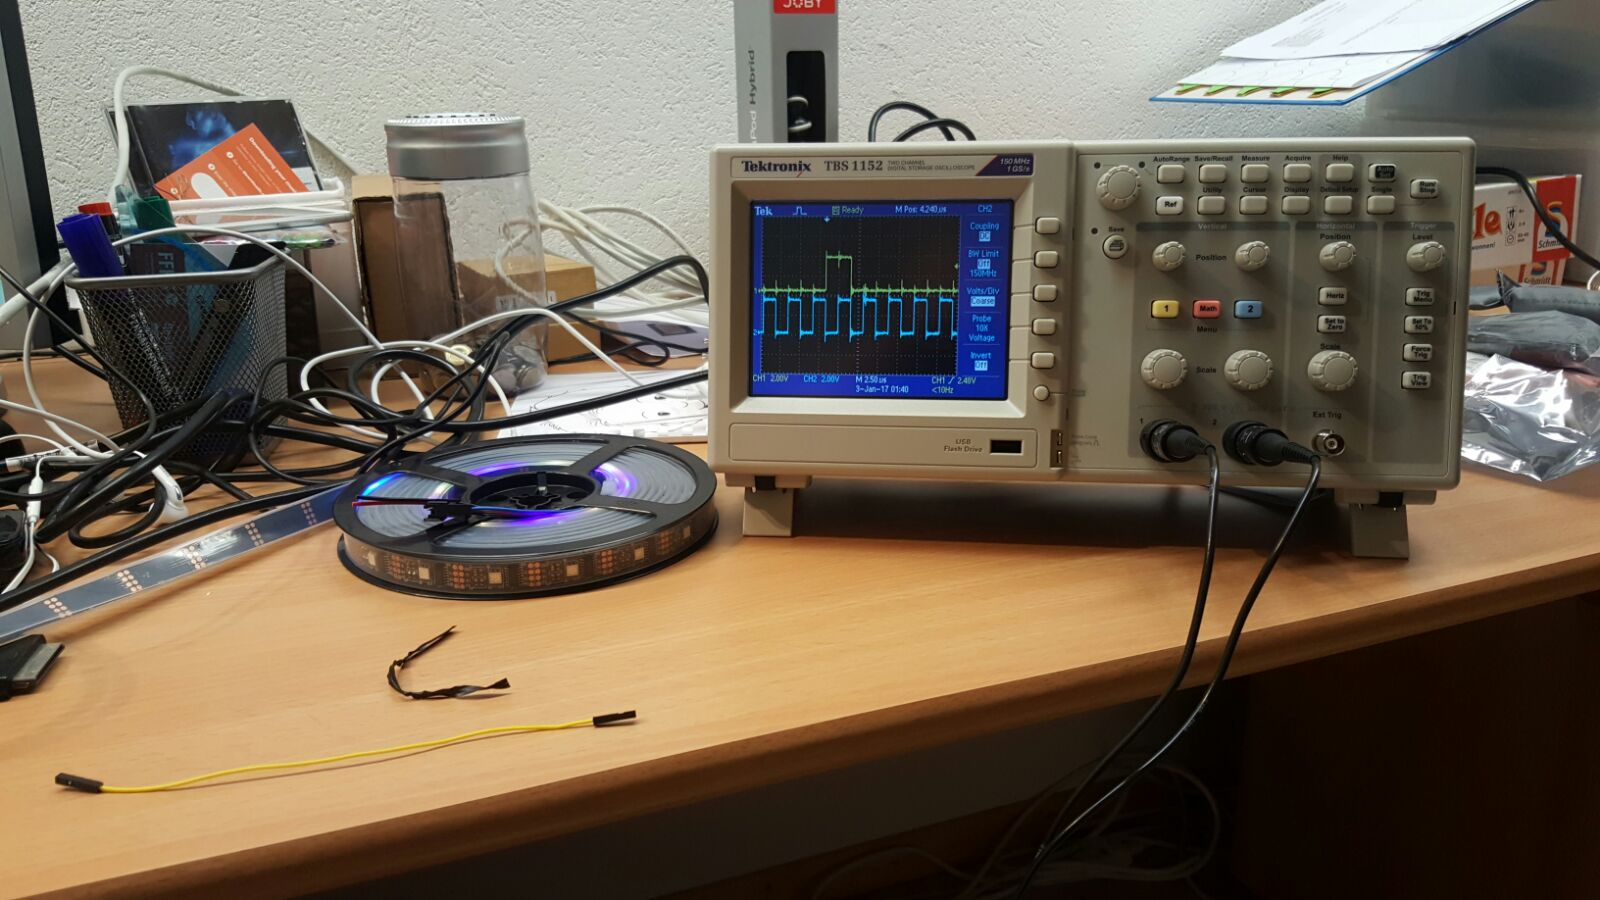
\includegraphics{../pictures/oszi.jpeg}
\caption{Hardwaretests}
\end{figure}

\subsection{Fazit}\label{fazit}

Das Projekt hat sich als sehr softwarelastig entpuppt. Die ursprüngliche
Idee, ein Wakeup-Light zu erstellen, hat sich schnell als relativ
einfach implementierbar herausgestellt. Komplexität gewann das Projekt
durch die Anforderung möglichst erweiterbar zu sein. Dieser Wunsch nach
Erweiterbarkeit schlug sich schnell im Softwaredesign nieder und
verursache erheblichen Mehraufwand in der Implementation. Die guten
libraries für den Raspberry PI haben sehr deutlich gezeigt, dass die
Hardware in einem solchen Projekt, nicht das Problem ist, sondern die
Software dahinter.

Obwohl der Hardwareteil etwas kleiner ausgefallen ist, als wir uns
ursprünglich vorgestellt haben, sind wir zufrieden mit unserem Resultat.
Das Projekt legt eine gute Basis für ein solides und erweiterbares
Weck-Automatisierungssystem.

\subsubsection{Projektmanagement}\label{projektmanagement-1}

Das Projekt Wakeup-Light wurde - ganz im Geiste des Fernstudiums -
komplett ``Remote'' umgesetzt. So konnten diverse Kollaborations-Tools
ausprobiert und direkt in den Projektablauf integriert werden. Ein gutes
Beispiel dafür ist der Projektplan, der mittels Google Docs online
geteilt wurde. Der Projektplan teilt das ganze Projekt in mehrere Work
Items - also kleine, überschaubare Arbeitseinheiten, die von einer
einzelnen Person umgesetzt werden können. Diese Work Items wurden dann
in Google Docs den Projektteilnehmern zugeteilt und dort auch
nachgeführt. Schlussendlich bestand das Projekt Wakeup-light aus über 50
Work Items.

Der Projektplan ist
\href{https://docs.google.com/spreadsheets/d/1FavRmBRhkSZag9ZJz7cpUHyRiqEvQwWesLXLay4Id8w/edit?usp=sharing}{hier}
einsehbar.

\subsubsection{Projektbeteiligung}\label{projektbeteiligung}

\begin{figure}[H]
\centering
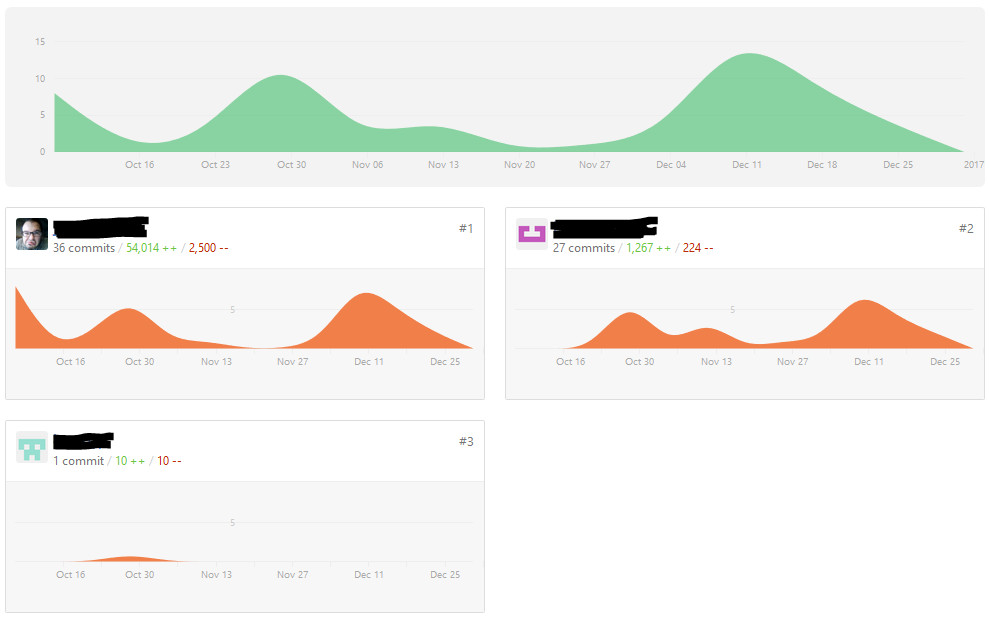
\includegraphics{./WI65_Kennzahlen.jpeg} 
\caption{Projektkennzahlen}
\end{figure}

Die Grafik zeigt den Beteiligungsverlauf der Projektteilnehmer. Die grünen Zahlen stellen die
hinzugefügten Anzahl Zeilen dar, während die Roten, die gelöschten
Zeilen darstellen. Die objektorientierten Analyse \& Design Dokumente
wurden in einem Format gespeichert, dass die grafischen Elemente
textuell beschreibt. So stehen diese Design Dokumente als Textdokumente
(JSON) zur Verfügung. Dies hat aber den Nachteil, dass mit der initialen
Erstellung dieser Dokumente eine enorm hohe Anzahl an Zeilen
(\textasciitilde{}36'000) erstellt wurden. Dieser Fakt zeigt sich in
dieser Endauswertung sehr deutlich.

\subsubsection{Ausfall Teammitglied}\label{ausfall-teammitglied}

Während des Projekts zeichnete sich sehr schnell ab, das nicht alle
Teilnehmer sich gleich stark beteiligen. E.M. hat erst gut gestartet und
innerhalb eines Tages das initiale Analysedokument durchgelesen und
Korrekturen angebracht. Danach ging es aber leider bergab mit seiner
Beteiligung. Die Bitte nach Feedback zu den Designdokumenten blieb
bereits unbeantwortet. Auf Rückfrage an der darauffolgenden Präsenz,
meinte dieser er habe die Dokumente zwar gesehen, sei dann aber in die
Ferien bis nach dem Abgabetermin. Daraufhin wurde vereinbart, dass jeder
Projektteilnehmer einen wöchentlichen Status zu seinen Arbeiten abgeben
soll. Jeweils auf Rückfrage, schickte E.M. auch einen kurzen Status, die
den anderen Projektteilnehmern Hoffnung gab, ``dass er einfach kein
grosser Redner ist, aber seine Arbeit macht''. Da bereits während der
Präsenz durchsickerte, dass E.M. mit der Designentscheidung SOAP als Web
Service Architektur zu verwenden, nicht ganz zufrieden war, wurde dies
nachträglich zur REST-Architektur geändert, in der Hoffnung, dass
dadurch die Beteiligung von E.M. steigen würde. Dieser bedankte sich per
E-Mail für diese Änderung und gab an, an der Implementierung eines
REST-Clients für den GUI Teil sei. In der darauffolgenden Woche, gab
E.M. - wieder erst auf Rückfrage - in seinem Status bekannt, dass er den
Client fertig hat und nun am Web-UI bzw. der
Schnittstellenimplementierung arbeiten will. Daraufhin wurde er per
E-Mail gebeten, seinen aktuellen Arbeitsstand jeweils in das Projekt
GIT-Repository hochzuladen - wie es die beiden anderen Projektteilnehmer
bereits seit Beginn der Arbeit tun - damit der Stand der Arbeit bewertet
werden kann. Ab diesem Zeitpunkt fand keine Kommunikation mehr statt.
Die restlichen Projektteilnehmer informierten daraufhin den Dozenten und
als dieser E.M. auch nicht erreichen konnte, teilten sie die
verbleibenden Arbeiten so gut es ging unter sich auf.

E.M. war zuständig für die clientseitige Implementation der Applikation.
Dazu gehörte der GUI-Teil mit Anbindung an den Web Service. Dieser Teil
fehlt nun komplett. Grundsätzlich wäre das Projekt aber bereits anders
dimensioniert und aufgeteilt worden, wäre bereits am Anfang klar
gewesen, dass das Projekt mit zwei Personen umgesetzt werden muss.

Sollte es für Notwendig befunden werden, kann auf Nachfrage die ganze
E-Mail Kommunikation digital zur Verfügung gestellt werden.


\listoffigures

\subsection{Quellen}\label{quellen}


\begin{itemize}
\tightlist
\item
  {[}Gim{]} {[}Effects of artificial dawn on subjective ratings of sleep
  inertia and dim light melatonin
  onset.{]}(https://www.ncbi.nlm.nih.gov/pubmed/20653451)
\end{itemize}

\end{document}
